%%
%% (
%%  )\ )                             (
%%  (()/(   (            (             )\  )   (
%%   /(_))  ))\   (       ))\  (   (   (()/(   ))\
%%   (_))  /((_)  )\  )  /((_) )\  )\   ((_))/((_)
%%   | _ \(_))(  _(_/( (_) )  ((_)((_)  _| |(_))
%%   |   /| || || ' \))/ -_)/ _|/ _ \/ _` |/ -_)
%%   |_|_\ \_,_||_||_| \___|\__|\___/\__,_|\___|
%%

\documentclass{article}
\usepackage[utf8x]{inputenc}
\usepackage{amsmath}
%\usepackage{slashbox}
\usepackage{amsfonts}
\usepackage{amssymb}
\usepackage{graphicx} % Paquete para incluir imágenes en el documento LaTeX
\usepackage{hyperref}
\hypersetup{
  colorlinks=true,
  linkcolor=blue,
  filecolor=magenta,
  urlcolor=cyan,
}
\urlstyle{same}
\usepackage{varwidth}

\newcommand\tab[1][1cm]{\hspace*{#1}}

\usepackage{multirow}

\usepackage[a4paper,rmargin=1.5cm,lmargin=1.5cm,top=1.5cm,bottom=1.5cm]{geometry}

\usepackage{pdfpages}

\usepackage{xcolor}
\usepackage{minted}
\setminted[cpp]{frame=lines, framesep=2mm, baselinestretch=1.2, rulecolor=\color{black!80},
                bgcolor=DarkGray,fontsize=\normalsize}
\usemintedstyle[cpp]{monokai}
\setminted[python]{frame=lines, framesep=2mm, baselinestretch=1.2, rulecolor=\color{black!80}, bgcolor=DarkGray}
\usemintedstyle[python]{monokai}
\setminted[java]{frame=lines, framesep=2mm, baselinestretch=1.2, rulecolor=\color{black!80}, bgcolor=DarkGray}
\usemintedstyle[java]{monokai}
\setminted[javascript]{frame=lines, framesep=2mm, baselinestretch=1.2, rulecolor=\color{black!80}, bgcolor=DarkGray}
\usemintedstyle[javascript]{monokai}
\setminted[php]{frame=lines, framesep=2mm, baselinestretch=1.2, rulecolor=\color{black!30}, bgcolor=LightGray}
\setminted[html]{frame=lines, framesep=2mm, baselinestretch=1.2, rulecolor=\color{black!30}, bgcolor=LightGray}
\setminted[bash]{baselinestretch=1.2,rulecolor=\color{black!30},fontsize=\footnotesize,bgcolor=LightGray}
\setminted[css]{frame=lines, framesep=2mm, baselinestretch=1.2, rulecolor=\color{black!80}, bgcolor=DarkGray}
\usemintedstyle[css]{monokai}
\definecolor{LightGray}{gray}{0.98}
\definecolor{DarkGray}{gray}{0.1}
\definecolor{MidGray}{gray}{0.8}
\definecolor{codegreen}{rgb}{0,0.6,0}
\definecolor{codegray}{rgb}{0.5,0.5,0.5}
\definecolor{codepurple}{rgb}{0.58,0,0.82}
\definecolor{backcolour}{rgb}{0.95,0.95,0.92}

\setlength{\parindent}{0px}  % Setea la indentacion de la primera linea de cada parrafo a cero pixeles.


\title{Introducción a JavaSE}
\author{@RuneCode}

\begin{document}
%% Portada
\includepdf{./portada/portada.pdf}

%% Clase 1
\section{¿Qué es Git?}%
Git es un software de control de versiones diseñado por Linus Torvalds,
pensando en la eficiencia y la confiabilidad del mantenimiento de versiones de
aplicaciones cuando estas tienen un gran número de archivos de código fuente.
En su lugar GitHub es una forja para alojar proyectos utilizando el sistema de
control de versiones Git. GitHub sería la red social de código para los
programadores, tu propio curriculum vitae.\\

%% Clase 2
\section{¿Por qué usar un sistema de control de versiones como Git?}%
Un sistema de control de versiones como Git nos ayuda a guardar el historial de
cambios y crecimiento de los archivos de nuestro proyecto.\\

En realidad, los cambios y diferencias entre las versiones de nuestros proyecto
pueden tener similitudes, algunas veces los cambios pueden ser solo una palabra
o una parte específica de un archivo específico. Git está optimizado para
guardar todos estos cambios de forma atómica e incremental, o sea, aplicando
cambios sobre los últimos cambios, estos sobre los cambios anteriores y así
hasta el inicio de nuestro proyecto.\\

Imagina que estás escribiendo tu biografía y en tu biografía escribes cosas
como:

\begin{figure}[h!]
  \centering
  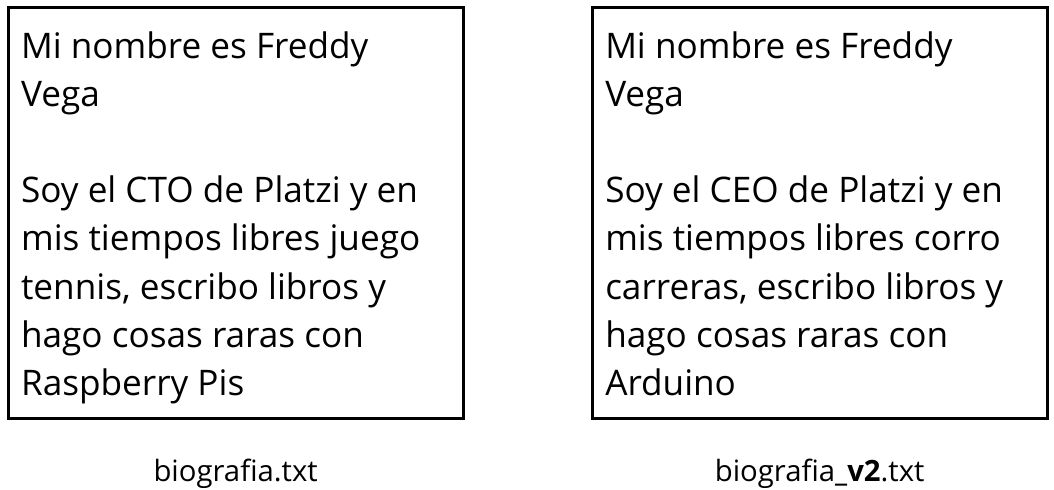
\includegraphics[scale=0.5]{./Pictures/001_no_git_example.png}
\end{figure}


Lo normal es que guardes los cambios en diferentes archivos poniéndoles nombres
diferentes como se vió en los ejemplos, y es lo que todos hacemos, sea en el
mundo del diseño o del márketing, programación. Antes de conocer los sistemas
de control de versiones esa era nuestra única opción.\\

Sin embargo es que son pocos los cambios ocurridos en nuestro archivo, y no
deberíamos guardar todo el archivo de nuevo solo por esos cambios. Es ideal el
hecho de poder guardar solo los cambios realizados, en especial cuando estamos
trabajando con múltiples personas sobre el mismo archivo o si estamos cambiando
pequeñas cosas sobre algo tan grande como por ejemplo el código de un proyecto
de software.

\begin{figure}[h!]
  \centering
  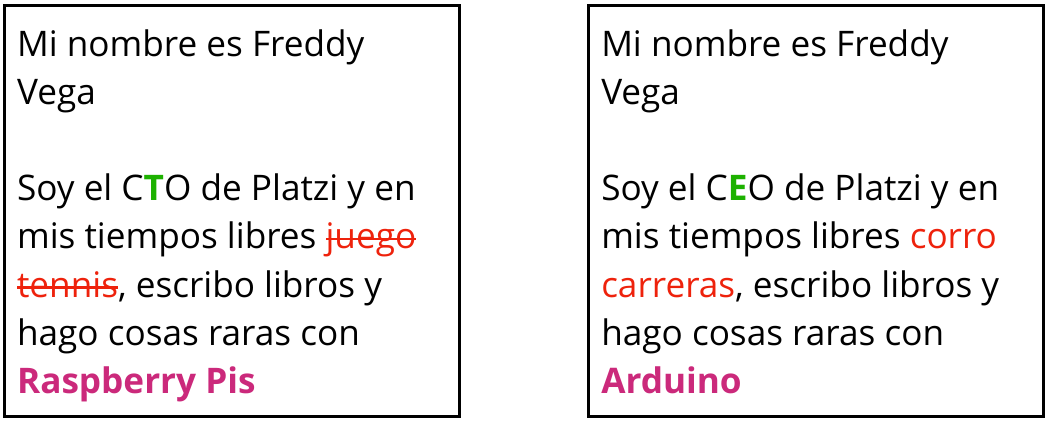
\includegraphics[scale=0.5]{./Pictures/002_solo_cambios.png}
\end{figure}

Aquí es donde entran los llamados \textbf{Sistemas de Control de
versiones}, que solo guardan esos cambios y dejar en claro donde ocurrieron,
cuando ocurrieron, quien los hizo, podemos volver a ellos en el pasado, entre
muchas otras cosas. El sistema de Control de versiones que vamos a ver en este
curso es el más popular del mundo se llama \textbf{Git}, fue creado por la
Fundación Linux, particularmente por Linus Torvalds, es el sistema que maneja
el kernel de Linux, y como vemos en la imágen, precisamente solo guarda los
cambios.

\begin{figure}[h!]
  \centering
  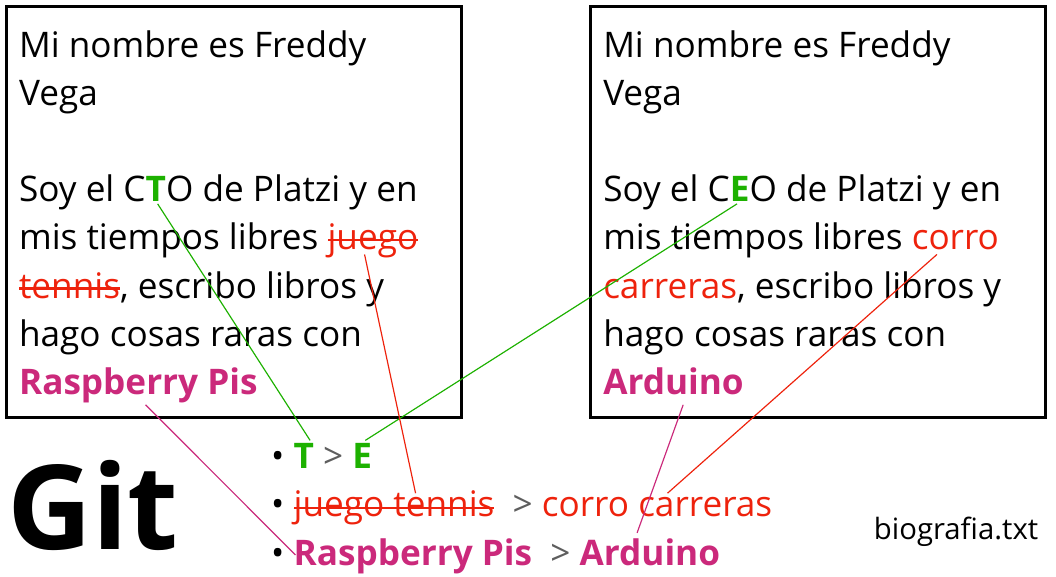
\includegraphics[scale=0.5]{./Pictures/003_git.png}
\end{figure}

Ahora seamos mucho más precisos con esto. Imaginémonos que tienes una carpeta
que es tu proyecto biografía donde tienes el archivo \textbf{biografia.txt}, un
archivo de texto plano. Texto plano es un archivo en el que no se puede guardar
estilos como negrita, cursiva, etc. Por esto un archivo de Word \textbf{.docx}
no es un archivo de texto plano, tampoco un \textbf{.rtf}. Pero un archivo
\textbf{.txt} tienden a ser un archivo de texto plano. La extensión como tal no
determina si un archivo es de texto plano, sino su composición interna.
Básicamente si lo habres en un \textbf{bloc de notas} o un editor de código y
es simplemente texto, es texto plano.

\begin{figure}[h!]
  \centering
  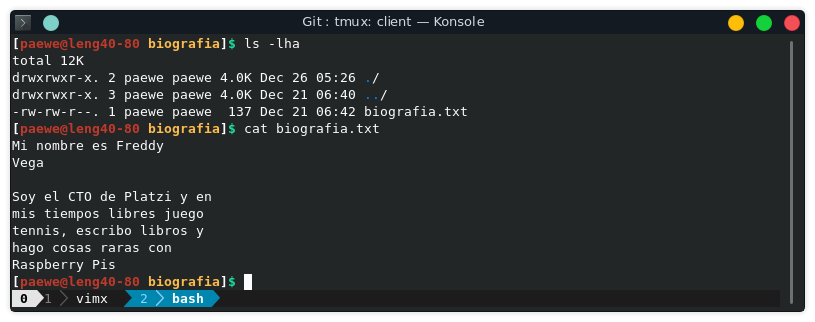
\includegraphics[scale=0.75]{./Pictures/004_biografiatxt.png}
\end{figure}

Entramos a la carpeta en la que tienes el archivos desde línea de comandos e
inicializamos el repositorio local.

\begin{figure}[h!]
  \centering
  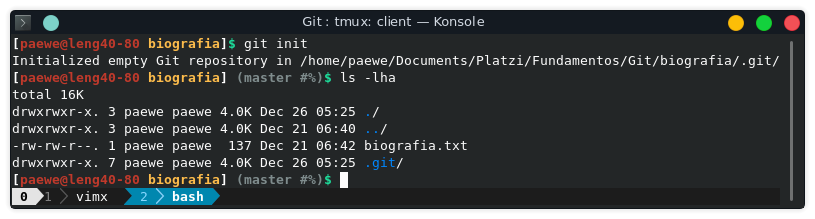
\includegraphics[scale=0.75]{./Pictures/005_gitinit.png}
\end{figure}

Pero ahora tu repositorio tiene que saber que este archivo existe, entonces
agregamos el archivo al \textbf{staging area} usando \textbf{git add} espacio el
nombre del archivo, con esto la base de datos de cambios del sistema de control
de versiones git ahora sabe que existe biografia.txt. Pero no basta con esto,
usamos \textbf{git commit} para enviar los cambios a la base de datos del
sistema de control de versiones y con \textbf{-m} se puede enviar un mensaje
entre comillas, esto es una buena práctica.

\begin{figure}[h!]
  \centering
  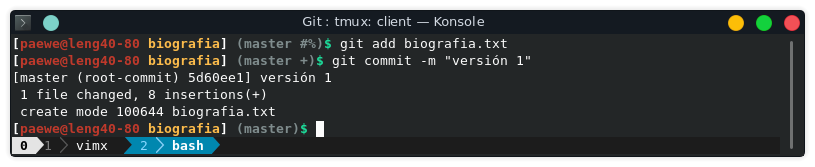
\includegraphics[scale=0.75]{./Pictures/005_version1.png}
\end{figure}

Ahora que tengo agregado este archivo voy al editor de texto y hago los
cambios.

\begin{figure}[h!]
  \centering
  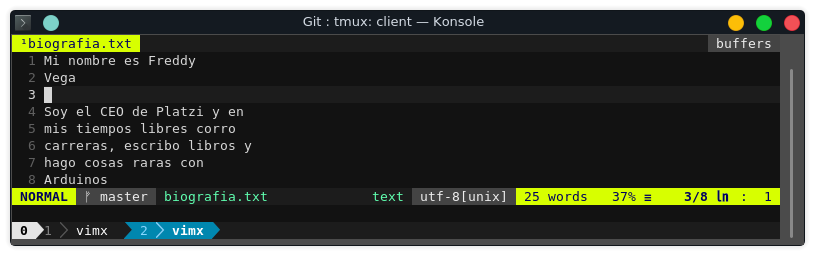
\includegraphics[scale=0.75]{./Pictures/006_editor.png}
\end{figure}

\begin{figure}[h!]
  \centering
  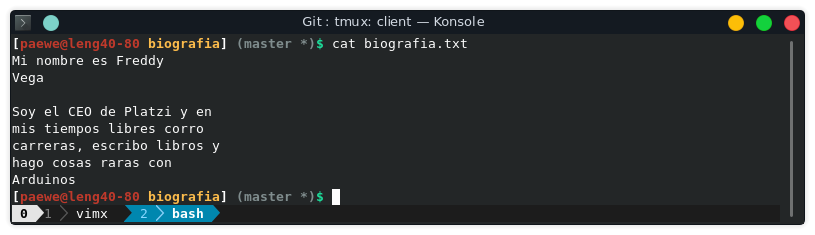
\includegraphics[scale=0.75]{./Pictures/006_cambios.png}
\end{figure}

Luego de guardar los cambios, estos están guardados en el disco duro, pero aún
no en mi repositorio. Para esto puedo usar \textbf{git add} con el nombre del
archivo nuevamente o también con \textbf{punto} que lo que hace es agregar
todos los archivos con cambios desde el directorio actual.
Una vez añadido esos cambios del archivo al staging, volvemos a hacer un commit.

\begin{figure}[h!]
  \centering
  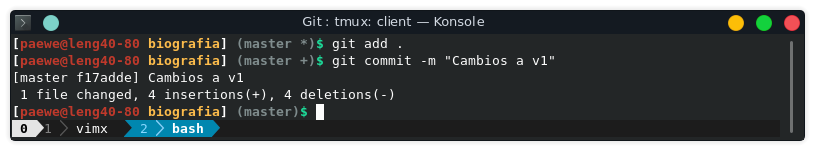
\includegraphics[scale=0.75]{./Pictures/007_gitcommit.png}
\end{figure}

Puedes ver el estado de tu repositorio haciendo uso de \textbf{git status}. Si
has hecho un cambio, pero no lo has añadido ahi te va a salir, si todo te está
bien entonces te va a decir que no hay problema.

\begin{figure}[h!]
  \centering
  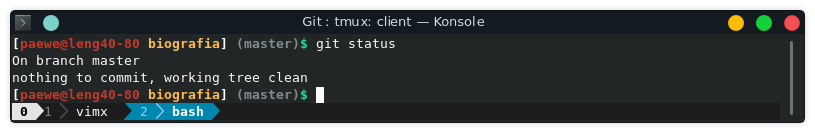
\includegraphics[scale=0.75]{./Pictures/008_gitstatus.png}
\end{figure}

Tenemos \textbf{git show} que muestra todos los cambios históricos hechos
incluyendo cuales han sido las líneas de código o de texto que hayan cambiado,
cuando y quien los hizo, porque a un repositorio pueden acceder múltiples
personas.

\newpage

\begin{figure}[h!]
  \centering
  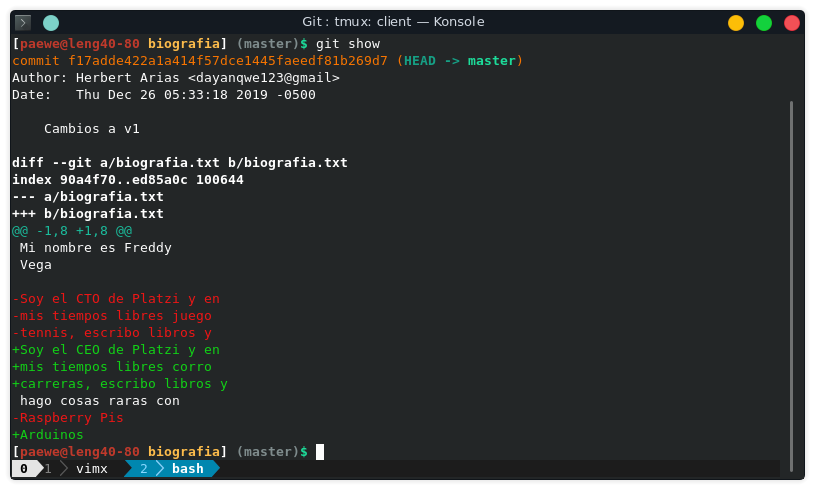
\includegraphics[scale=0.75]{./Pictures/009_gitshow.png}
\end{figure}

También si quieres ver la historia completa de un archivo, puedes usar
\textbf{git log}

\begin{figure}[h!]
  \centering
  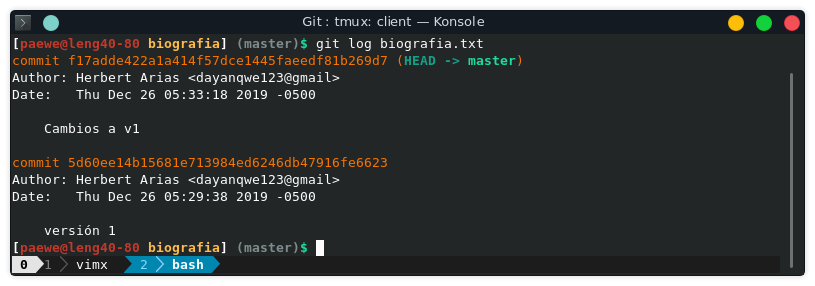
\includegraphics[scale=0.75]{./Pictures/010_gitlog.png}
\end{figure}

Por último si ya estás listo y has completado todos estos pasos, quizás puedes
llevar tu repositorio a un servidor remoto, porque probablemente ese archivo
vive en un repositorio en internet o en un servidor donde tu quieres que lo vea
todo el mundo. Eso lo vamos a ver más adelante en el curso y es el comando
\textbf{git push}. Y estos son los comandos básicos de git.

\begin{figure}[h!]
  \centering
  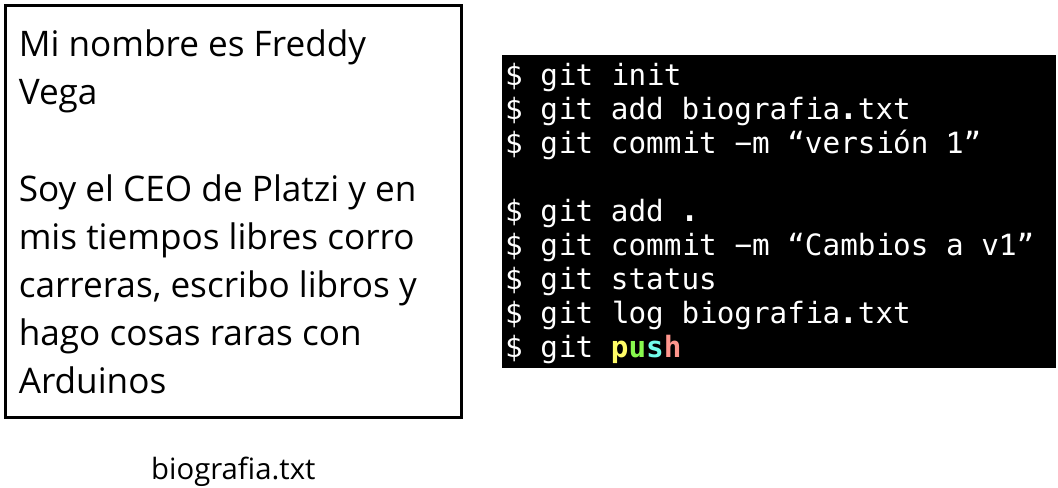
\includegraphics[scale=0.5]{./Pictures/011_basicos.png}
\end{figure}

\newpage

%% Clase 3
\section{Instalando Git y GitBash en Windows}%
En Windows lo primero que tienes que hacer es instalar git. Entonces vamos al
\href{https://git-scm.com/}{enlace}, ahí vamos a encontrar la versión de git
oficial. Git es creado por la fundación que hace Linux, de hecho es creado por
Linus Torvalds.

\begin{figure}[h!]
  \centering
  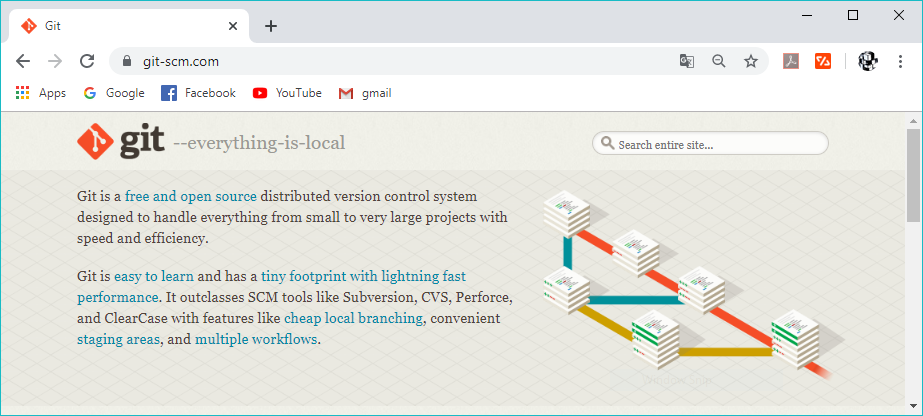
\includegraphics[scale=0.5]{./Pictures/011_gitbash.png}
\end{figure}

Entonces le damos en descargar.

\begin{figure}[h!]
  \centering
  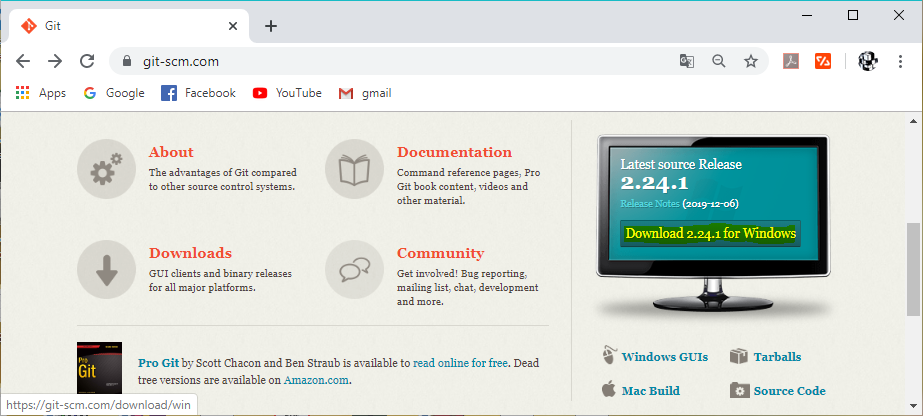
\includegraphics[scale=0.5]{./Pictures/012_gitbash.png}
\end{figure}

Luego de la descarga vamos a abrirlo e instalarlo. Es el típico instalador de
Windows donde le das next, next.

\begin{figure}[h!]
  \centering
  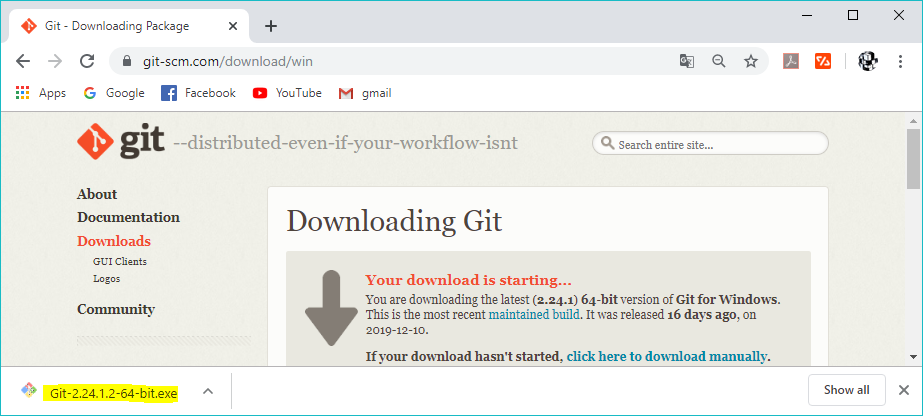
\includegraphics[scale=0.5]{./Pictures/013_gitbash.png}
\end{figure}

\newpage

\begin{figure}[h!]
  \centering
  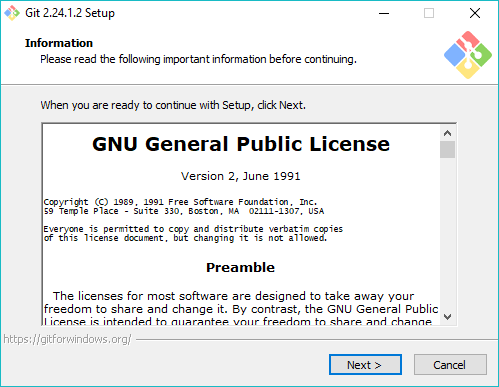
\includegraphics[scale=0.65]{./Pictures/014_install_git.png}
\end{figure}

En esta sección asegúrate que donde dice \textbf{Git Bash Here} esta remarcado
para que se instale, el resto lo dejamos igual. También puedes remarcar la
opción que verifica nuevas versiones para Windows o también la opción para usar
\textbf{TrueType} para que muestre las fuentes mucho más suaves en la línea de
comando. Luego Next.

\begin{figure}[h!]
  \centering
  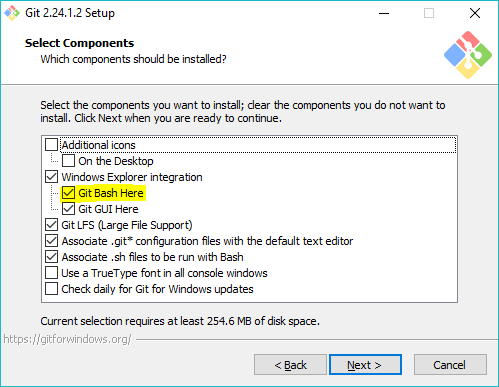
\includegraphics[scale=0.65]{./Pictures/015_install_git.png}
\end{figure}

Luego nos aparece la opción para cambiar el editor Vim por otro. Por el momento
lo dejamos así. Luego lo vamos a modificar, solamente como referencia esta es
una forma para cambiar el editor visual por defecto de git. Y le damos next.

\begin{figure}[h!]
  \centering
  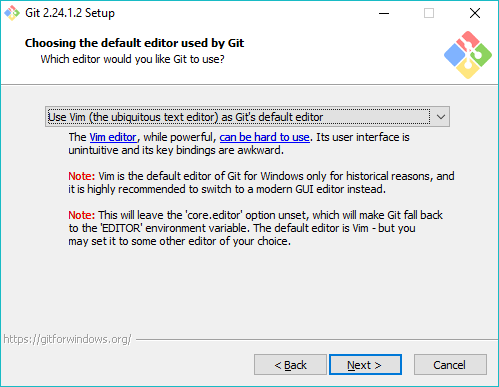
\includegraphics[scale=0.65]{./Pictures/016_install_git.png}
\end{figure}

\newpage

Estas opciones basicamente tienen que ver con que Windows no es un entorno
\textbf{"amigable"} para programadores. Los programadores normalmente usan
Linux o Sistemas basados en UNIX como MAC para poder trabajar, porque todos sus
comandos están basados en esta terminal. La terminal de Linux y UNIX.\\

Si tu estás en Windows, no te preocupes, \textbf{Git} instala algo que se llama
\textbf{Gitbash} que te va hacer la vida más facil, pero también se puede usar
Git desde la línea de comandos nativa de Windows (DOS).\\

En esta parte tienes que decidir entre usar git solo desde la terminal emulada
de Linux que te va a instalar el sistema en Windows o si lo quieres usar desde
cualquier parte. Realmente no hay nada que perder si usamos esta segunda
opción, es decir que se pueda usar desde la línea de comandos que ya es nativa
en Windows y además desde el software como Gitbash entre otros.

\begin{figure}[h!]
  \centering
  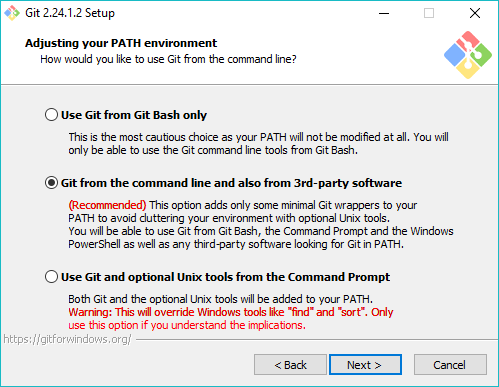
\includegraphics[scale=0.65]{./Pictures/017_install_git.png}
\end{figure}

Luego nos está preguntando que tipo de librería vamos a usar para la seguridad.
Esto también es importante, porque en el mundo UNIX, Linux y MAC. Ya está
instalado un sistema de seguridad que se llama OpenSSL, si tu has escuchado de
SSH, SSL o de llaves públicas y privadas habrás escuchado de esta librería.
Cuando tu entras a un sitio web seguro HTTPS lo que haces es intercambiar unas
llaves de criptografía en vez de simplemente una contraseña, para que toda tu
información esté cifrada y protegida, eso se hace con \textbf{OpenSSL}, pero
esta es una librería que no está instalada por defecto en Windows.\\

En Windows si hay unas librerías que se llaman \textbf{Windows Certificate
Stores and Internal Root CA certificates}, que es básicamente una forma en la
cual ellos manejan la seguridad a nivel de Microsoft, no es que sea malo, es
que es distinto y la gran mayoría del mundo del desarrollo de software usan
OpenSSL.

Si no quieres preocuparte y si quieres que tu vida sea facil, elige la primera
opción \textbf{Use the OpenSSL library} y dale clic en Next ;)

\begin{figure}[h!]
  \centering
  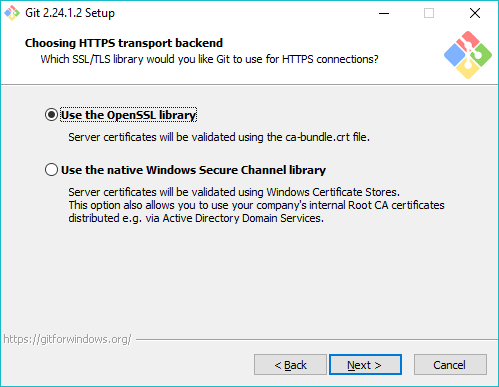
\includegraphics[scale=0.65]{./Pictures/018_install_git.png}
\end{figure}

Windows y Linux guardan el \textbf{Enter} de manera distinta. En las tres
opciones que muestra la siguiente captura simplemente te estan preguntado
¿Quieres que nos encarguemos nosotros?, ¿Te encargas tú? o se lo encomendamos a
Dios, xd. Esas son las tres opciones.\\

En la primera opcion: Al principio se reciben los saltos en línea a la manera
en Windows y luego cuando se envían al repositorio se convierten a la manera de
Linux o de Unix.\\
En la segunda opción: Es como caiga, como se encuentre en el sistema
operativo.\\
Y en la tercera opción: No hace conversiones tampoco, entonces puede que genere
inconvenientes.\\

Normalmente en un entorno de desarrollo de verdad van haber personas que usen
Windows, Linux o Mac. Entonces la primera opción es la que te hace más
compatible con todo el mundo.

\begin{figure}[h!]
  \centering
  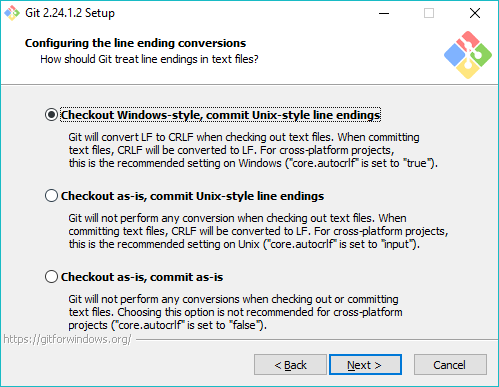
\includegraphics[scale=0.65]{./Pictures/019_install_git.png}
\end{figure}

Ahora te pregunta Git si quieres usar el sistema de Windows CMD o su emulador
de Linux que se llama MinTTY, que es la terminal por defecto del sistema que
emula Linux dentro de Windows. Yo creo que lo mejor es que elijan la opción
\textbf{Use MinTTY} porque así te acostumbras como funciona la terminal y la
verdad es que incluso programadores que usan Windows, excepto que sean
programadores de cosas como \textbf{.NET} o el entorno normal de Microsoft, van
a estar usando comandos de Linux que es lo más común del mundo. De hecho ya se
puede instalar Ubuntu en Windows. Si tu tienes Windows 10 puedes ir a la tienda
de aplicaciones de Windows, buscar Ubuntu e instalarlo y te abre una consola
completa de Linux con el Kernel de Linux, no emulado sino corriendo en paralelo
a Winows, es fascinante pero no es el alcance de este curso.\\

\begin{figure}[h!]
  \centering
  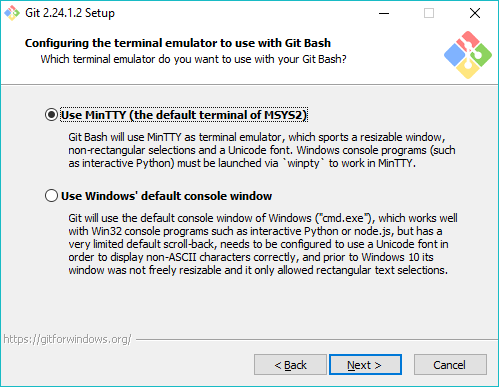
\includegraphics[scale=0.65]{./Pictures/020_install_git.png}
\end{figure}

\newpage

Luego nos quedan configuraciones extras como el de activar los \textbf{enlaces
simbólicos} que son como los \textbf{accesos directos} de Windows pero que
funcionan en Linux, podemos activarlo si queremos.\\

Git Credential Manager, es una forma en la que se manejan y se guardan las
llaves privadas de Git, pero funcionando dentro del mundo de Windows. File
system caching es simplemente una forma de hacer que todo corra mucho más
rápido porque se va a guardar dentro del caché del sistema.


\begin{figure}[h!]
  \centering
  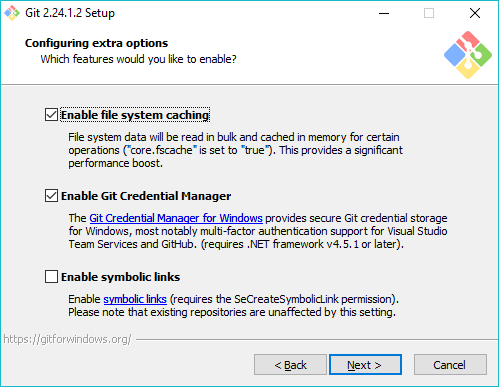
\includegraphics[scale=0.65]{./Pictures/021_install_git.png}
\end{figure}

Por último \textbf{install}.

\begin{figure}[h!]
  \centering
  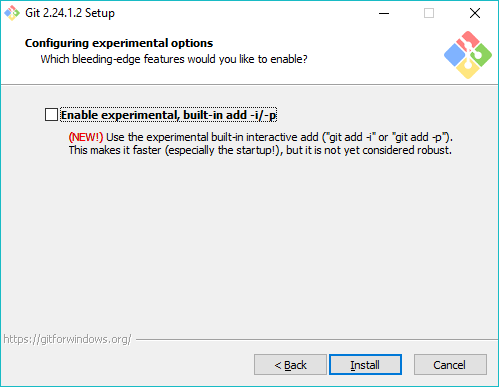
\includegraphics[scale=0.65]{./Pictures/022_install_git.png}
\end{figure}

Luego de terminar la instalación en el asistente desmarcamos \textbf{View
Release Notes}, ya que muestra los últimos cambios hechos en Git. Pero marcamos
\textbf{Launch Git Bash} que sí nos interesa. Nos va abrir una consola interna
que pareciera de Linux. En esta consola se pueden usar algunos comandos
Linux.\\

\begin{figure}[h!]
  \centering
  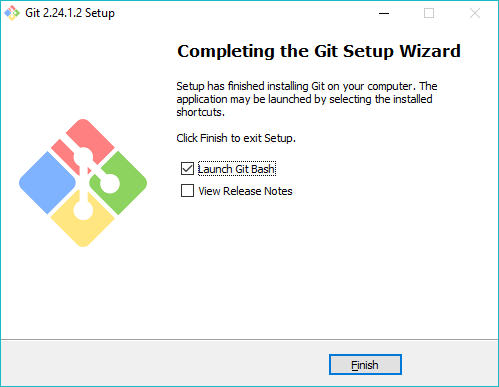
\includegraphics[scale=0.65]{./Pictures/023_install_git.png}
\end{figure}

Para abrirlos de nuevo, lo único que tienes que hacer es presionar la tecla
Windows y buscar la palabra git y te devolverá en la búsqueda Git Bash.

\newpage

%% Clase 4
\section{Instalando Git en OSX}%
En un Mac la historia es muy similar. Escribes git en safari, luego ingresas a
\textbf{git-scm.com}, le das scroll y mira como el sistema detecta
automáticamente que estás en Mac. Le das clic en descargar.

\begin{figure}[h!]
  \centering
  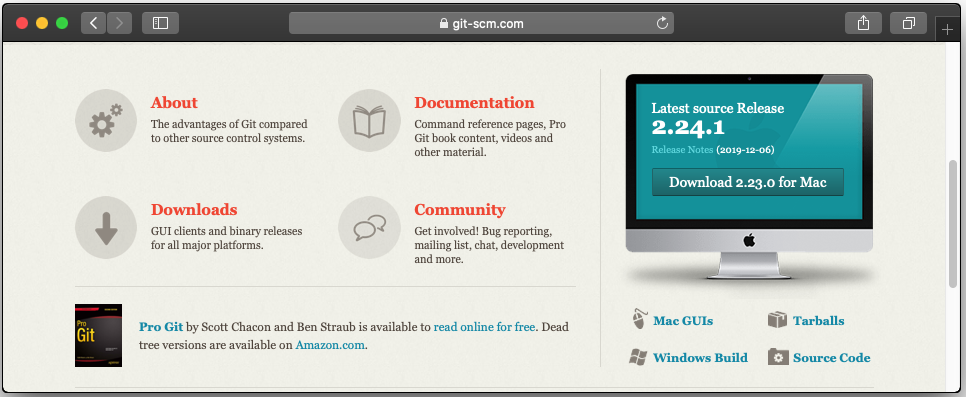
\includegraphics[scale=0.5]{./Pictures/022_mac_git.png}
\end{figure}

\begin{figure}[h!]
  \centering
  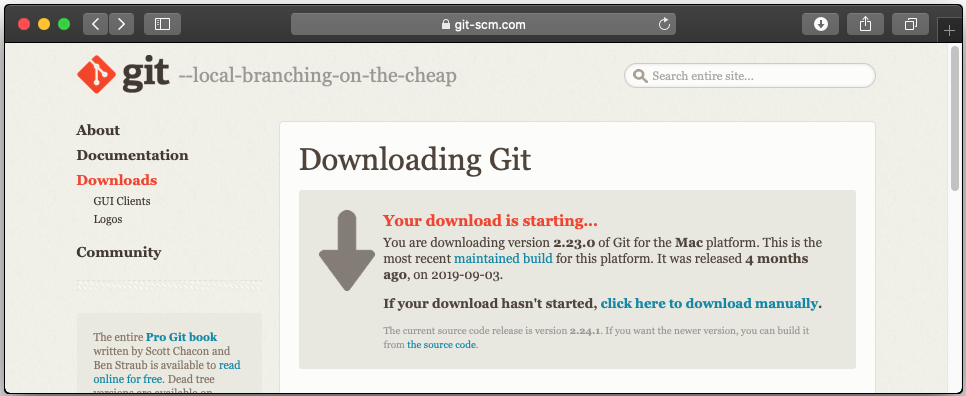
\includegraphics[scale=0.5]{./Pictures/023_mac_git.png}
\end{figure}

Se descargará un archivo que tiene una extensión \textbf{.dmg}, estos son los
archivos típicos de instalación dentro del mundo de Mac. DMG es el archivo
estandar dentro del mundo Mac para colocar archivos de instalación.

\begin{figure}[h!]
  \centering
  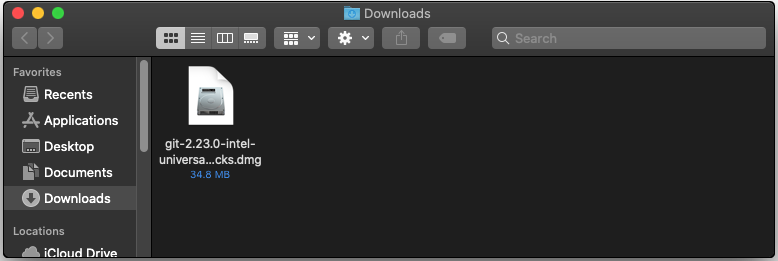
\includegraphics[scale=0.5]{./Pictures/024_mac_git.png}
\end{figure}

Le das abrir y abrirá un paquete de instalación. Para instalar un software en
ocasiones en Mac tu arrastras y sueltas y en otras ocasiones tienes que darle
doble clic. Entonces en este caso tu sabes que le das doble clic porque te sale
una caja amarilla con una extensión \textbf{.pkg}.

\newpage

\begin{figure}[h!]
  \centering
  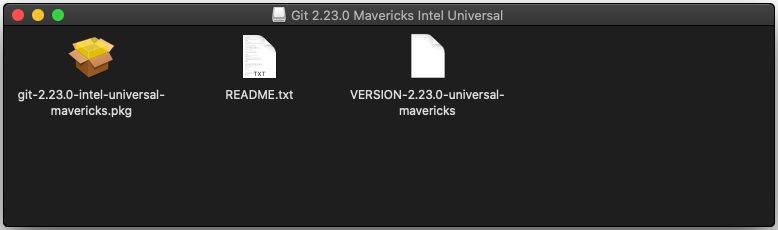
\includegraphics[scale=0.5]{./Pictures/025_mac_git.png}
\end{figure}

Si le das doble clic para instalarlo, te va a salir un error de este estilo,
diciéndote que no puede ser abierto porque es de un desarrollador no
identificado. En algunos casos te va a salir, en otros no.

\begin{figure}[h!]
  \centering
  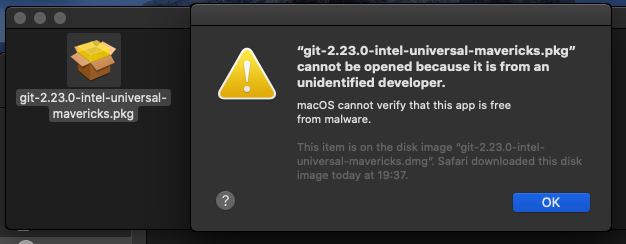
\includegraphics[scale=0.5]{./Pictures/026_mac_git.png}
\end{figure}

Si te sale simplemente le das clic derecho y open. Y ahora si en el cuadro de
diálogo te sale la opción de open, esta es una opción de seguridad que tiene
Mac para saber que estás haciendo lo correcto. Ahora si le das clic en Open
ahora sí entonces te va a abrir el instalador, que se parece mucho al installer
de Windows. Simplemente le das continue e install. En algun punto te va a pedir
tu contraseña de usuario.

\begin{figure}[h!]
  \centering
  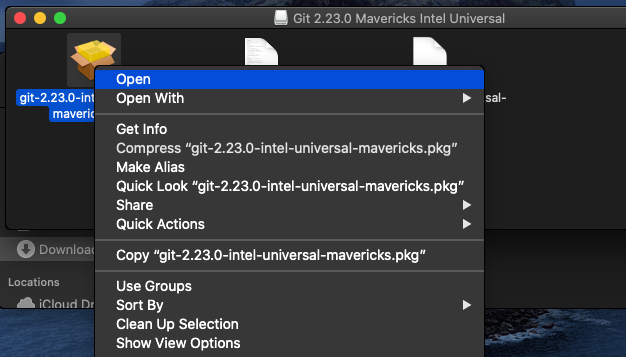
\includegraphics[scale=0.5]{./Pictures/027_mac_git.png}
\end{figure}

\begin{figure}[h!]
  \centering
  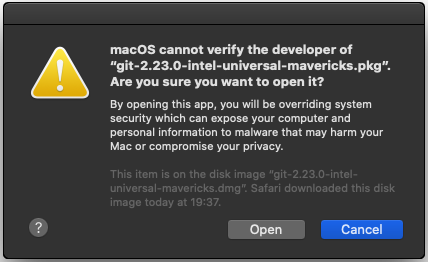
\includegraphics[scale=0.5]{./Pictures/028_mac_git.png}
\end{figure}

\newpage

\begin{figure}[h!]
  \centering
  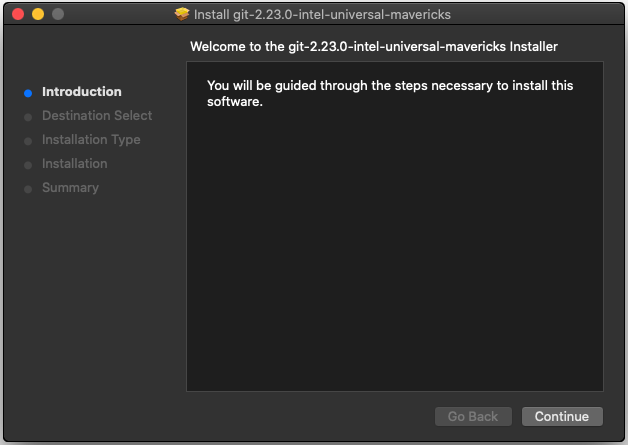
\includegraphics[scale=0.5]{./Pictures/029_mac_git.png}
\end{figure}

\begin{figure}[h!]
  \centering
  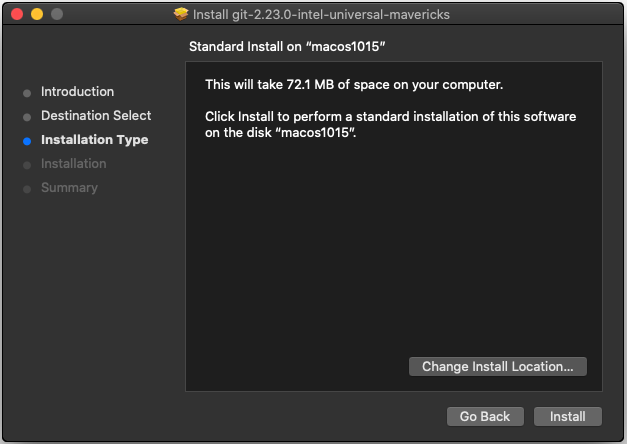
\includegraphics[scale=0.5]{./Pictures/030_mac_git.png}
\end{figure}

\begin{figure}[h!]
  \centering
  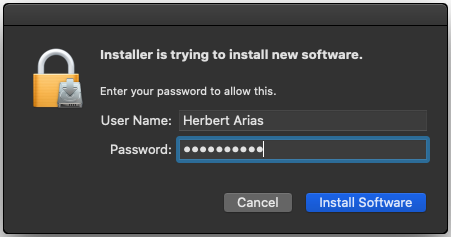
\includegraphics[scale=0.5]{./Pictures/031_mac_git.png}
\end{figure}

\newpage

\begin{figure}[h!]
  \centering
  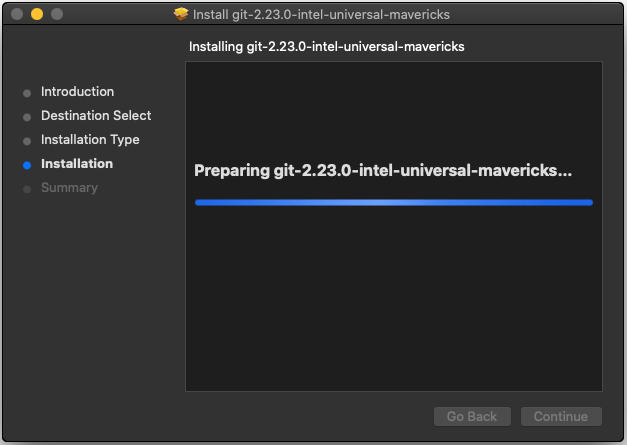
\includegraphics[scale=0.5]{./Pictures/032_mac_git.png}
\end{figure}

\begin{figure}[h!]
  \centering
  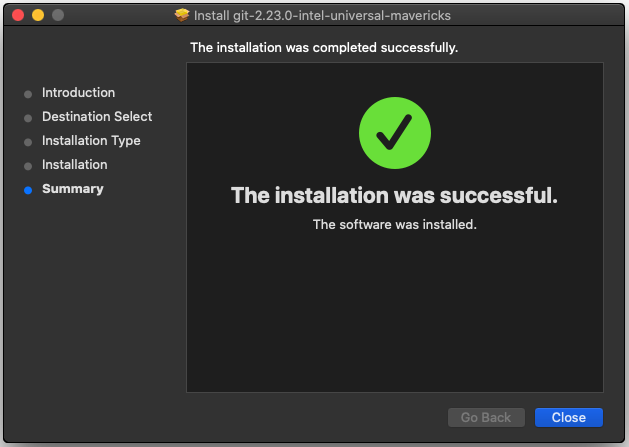
\includegraphics[scale=0.5]{./Pictures/033_mac_git.png}
\end{figure}

Le damos en Close y luego en Move to Trash que eliminará el instalador.

\begin{figure}[h!]
  \centering
  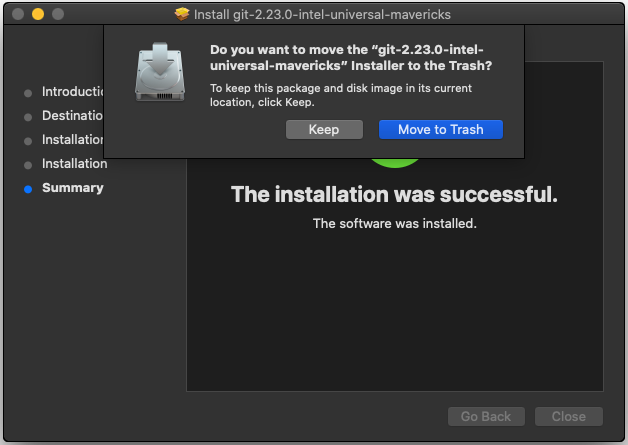
\includegraphics[scale=0.5]{./Pictures/034_mac_git.png}
\end{figure}

Pero aquí no te tuvo que instalar \textbf{gitbash} o configurar
\textbf{OpenSSL} ni nada de esas cosas porque en el mundo Mac al igual que en
el mundo Linux ya viene todo instalado por defecto, es el entorno tradicional
de un programador. En el mundo Mac tu ya tienes una terminal que se comporta
exáctamente igual a una terminal de UNIX o de Linux. Realmente no es
exactamente igual ya que Mac está basado en un Kernel que se llama BSD, donde
Linux está basado en Linux y tienen pequeñas diferencias y en el mundo práctico
no se ven a menos que estés haciendo cosas muy exóticas como acceso profundo a
las interfaces de red o acceso profundo a los archivos del sistema operativo.
En la práctica una consola de Mac y una de Linux son muy similares lo que sí es
muy distinto es una consola de Windows por eso emulamos Linux en Windows con
las consolas que instala Git.\\

En Mac no tienes instalado Git Bash, que se instala en Windows, porque ya
tienes una terminal, entonces lo que tienes que hacer es abrir la terminal y
ver que Git está instalado. Para esto nos vamos a la lupa que aparece en la
parte superior derecha y buscamos con la palabra \textbf{terminal}, luego
presionamos enter.

\begin{figure}[h!]
  \centering
  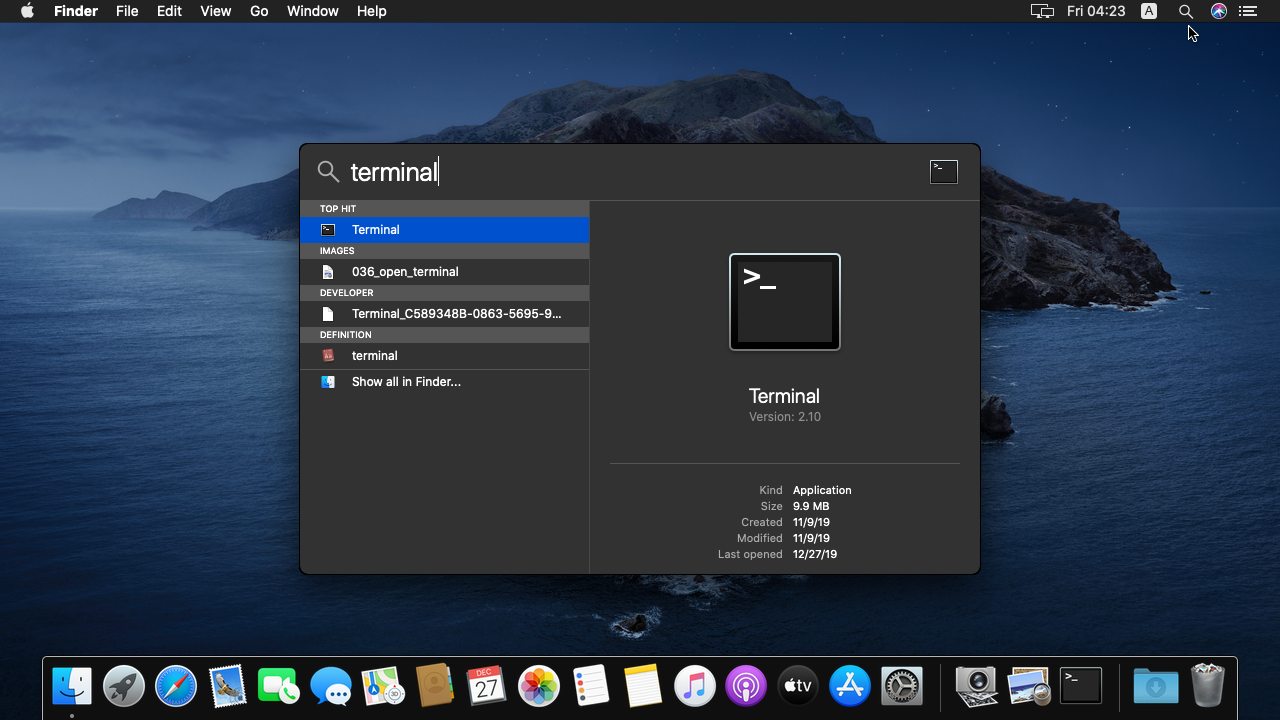
\includegraphics[scale=0.4]{./Pictures/037_terminal.png}
\end{figure}

En esta terminal entre muchas otras cosas podemos por ejemplo visualizar la
información de nuestro sistema.

\begin{figure}[h!]
  \centering
  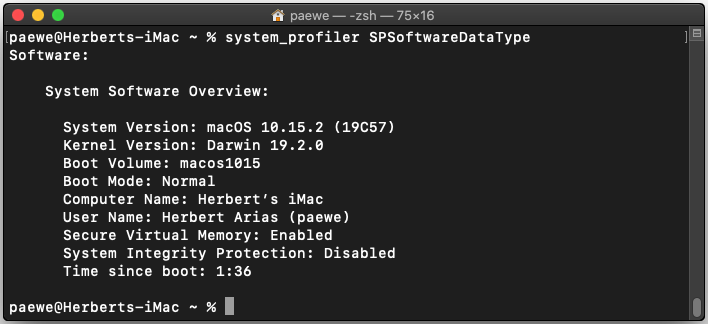
\includegraphics[scale=0.5]{./Pictures/036_mac_terminal.png}
\end{figure}

\newpage

Ahora vamos a verificar la instalación de Git.

\begin{figure}[h!]
  \centering
  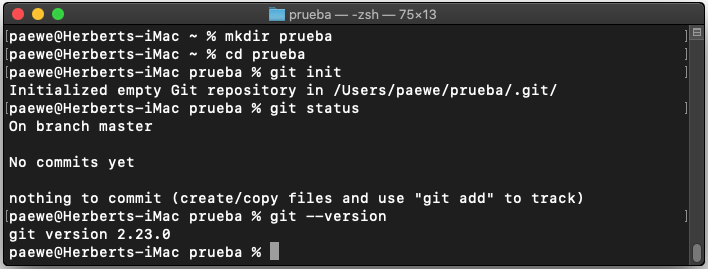
\includegraphics[scale=0.5]{./Pictures/035_mac_git.png}
\end{figure}

\newpage

%% Clase 5
\section{Instalando Git en Linux}%
Cada distribución de Linux tiene un comando especial para instalar herramientas
y actualizar el sistema.\\

En las distribuciones derivadas de Debian (como Ubuntu) el comando especial es
apt-get, en Red Hat es yum y en ArchLinux es pacman. Cada distribución tiene su
comando especial y debes averiguar cómo funciona para poder instalar Git.\\

Antes de hacer la instalación, debemos hacer una actualización del sistema. En
nuestro caso, los comandos para hacerlo son sudo apt-get update y sudo apt-get
upgrade.\\

Con el sistema actualizado, ahora sí podemos instalar Git y, en este caso, el
comando para hacerlo es sudo apt-get install git. También puedes verificar que
Git fue instalado correctamente con el comando git --version.\\

La instalación en \textbf{Fedora} se realiza con el comando \textbf{dnf}.

\begin{minted}{bash}
  sudo dnf install git
\end{minted}

Con este único comando ya tendremos \textbf{git} instalado en nuestro sistema.
Para esto abriremos la terminal, hay muchas maneras de hacerlo. Una de la
formas de abrir la terminal en Fedora con entorno gráfico KDE es utilizando el
buscador, presionamos las teclas \textbf{ALT + F2} y luego escribimos
\textbf{konsole}, luego presionamos \textbf{enter}.

\begin{figure}[h!]
  \centering
  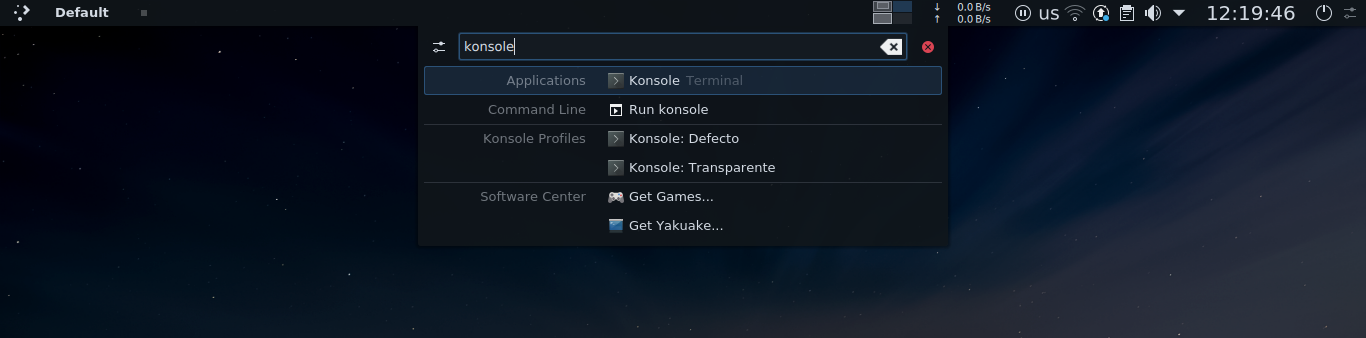
\includegraphics[scale=0.5]{./Pictures/038_fedora_terminal.png}
\end{figure}

Procedemos a usar el comando para instalar Git, nos muestra información de los
paquetes que se instalarán y escribimos \textbf{y} para aceptar y
\textbf{enter}. Luego de esto comenzará la descarga e instalación.

\begin{figure}[h!]
  \centering
  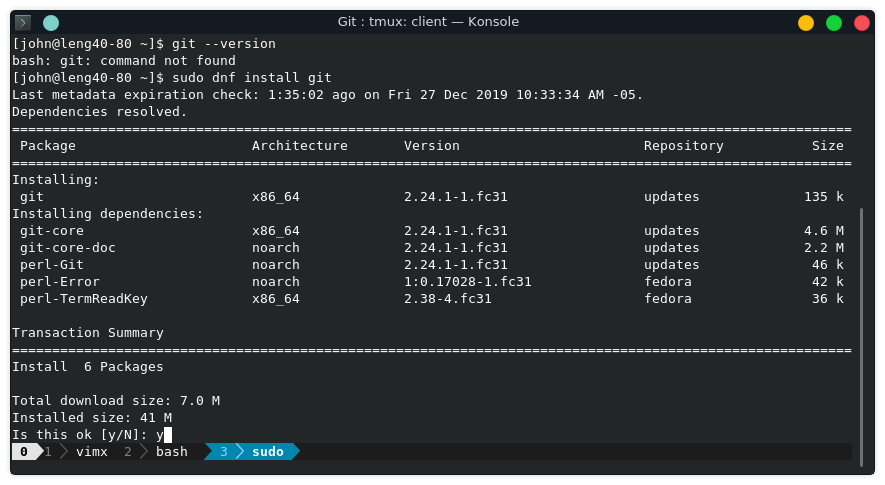
\includegraphics[scale=0.75]{./Pictures/039_fedora_install_git.png}
\end{figure}

\begin{figure}[h!]
  \centering
  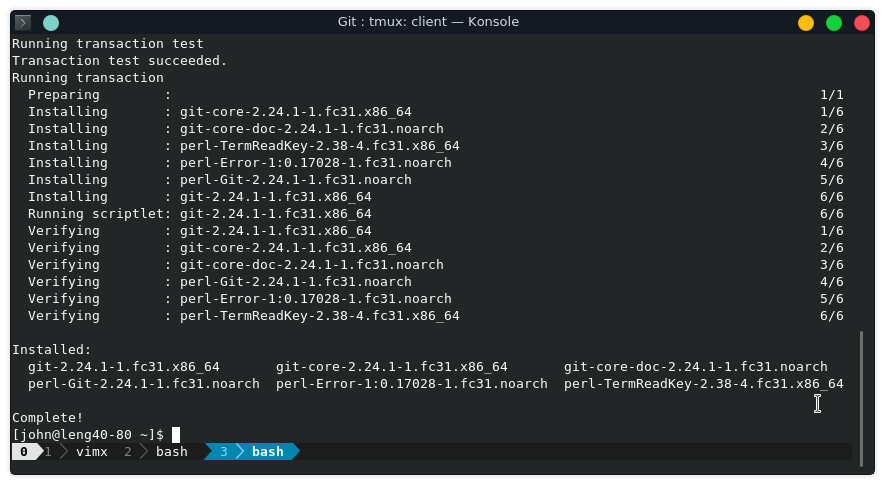
\includegraphics[scale=0.75]{./Pictures/040_fedora_install_complete.png}
\end{figure}

\newpage

Luego de terminar la instalación del paquete podemos verificar su instalación
verificando la versión de git.

\begin{minted}{bash}
  git --version
\end{minted}

\begin{figure}[h!]
  \centering
  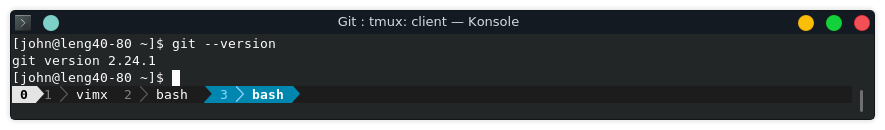
\includegraphics[scale=0.75]{./Pictures/041_git_installed.png}
\end{figure}

Ahora vamos a configurar nuestro prompt \textbf{bash} para que reconozca los
estados de git.\\

Primero configuraremos el prompt, esto se logra modificando la variable
\textbf{PS1} en el fichero .bashrc, sin embargo puedes usar el fichero
\href{https://raw.githubusercontent.com/xguestone/dotfiles/master/fedora/.bashrc}{.bashrc}
que tengo configurado para la distribución Fedora.\\

Primero hacemos un backup del fichero \textbf{.bashrc} que viene configurado en
nuestro home. Para esto nos ubicamos en el home, podemos hacerlo escribiendo el
comando \textbf{cd} y enter. Luego cambiamos el nombre actual del fichero
.bashrc usando \textbf{mv}.

\begin{minted}{bash}
  cd
  mv .bashrc .bashrc-bak
\end{minted}

Luego descargamos el fichero raw de
\href{https://raw.githubusercontent.com/xguestone/dotfiles/master/fedora/.bashrc}{.bashrc}
usando curl. Te dejo el enlace. Recuerda estar siempre trabajando en tu HOME.

\begin{minted}{bash}
  curl -o .bashrc https://raw.githubusercontent.com/xguestone/dotfiles/master/fedora/.bashrc
\end{minted}

\newpage

\begin{figure}[h!]
  \centering
  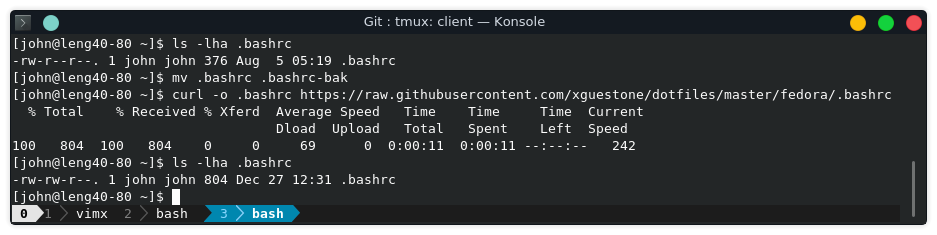
\includegraphics[scale=0.75]{./Pictures/042_bashr_ok.png}
\end{figure}


Git maneja un script bash para gestionar el prompt de acuerdo a sus estados,
este se encuentra en el mismo repositorio de \textbf{Git}. Encontramos el
script bash en formato \textbf{raw} en el siguiente
\href{https://raw.githubusercontent.com/git/git/master/contrib/completion/git-prompt.sh}{enlace}.\\

Creamos una carpeta llamada \textbf{shconf} dentro de \textbf{.config} y nos
ubicamos en esa carpeta.

\begin{minted}{bash}
  mkdir .config/shconf
  cd .config/shconf
\end{minted}

Ahora descargamos el fichero usando \textbf{wget} o \textbf{curl}.

\begin{minted}{bash}
  wget https://raw.githubusercontent.com/git/git/master/contrib/completion/git-prompt.sh
\end{minted}

Luego podemos activar los cambios realizados en \textbf{.bashrc} usando el
comando \textbf{source}.

\begin{minted}{bash}
  source ~/.bashrc
\end{minted}

\begin{figure}[h!]
  \centering
  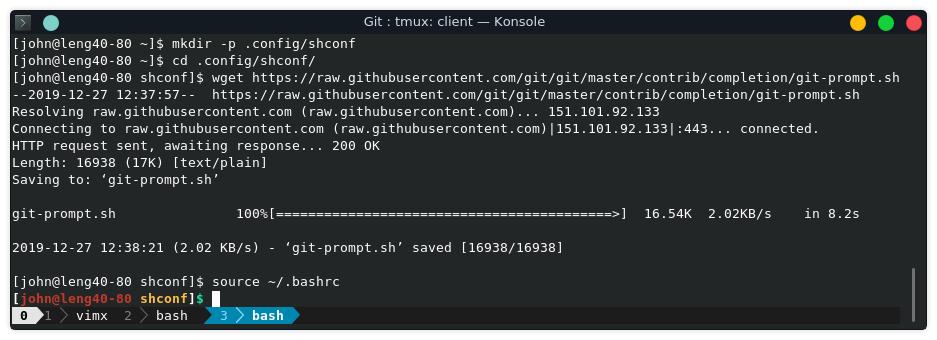
\includegraphics[scale=0.75]{./Pictures/043_bashrc_git_ok.png}
\end{figure}

Por último haremos una prueba de como cambia el prompt coforme los diferentes
estados de Git.

\begin{figure}[h!]
  \centering
  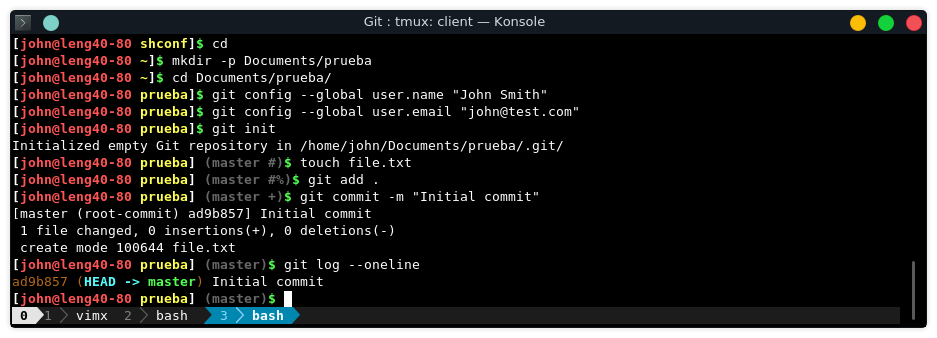
\includegraphics[scale=0.75]{./Pictures/044_git_funcional.png}
\end{figure}

\newpage


%% Clase 6
\section{Editores de código, archivos binarios y de texto plano}%
Vamos a instalar un editor de código, un editor de texto plano que nos permita
crear nuestros archivos del proyecto que querramos hacer durante el curso.\\

¿Por qué un editor de código? Porque es distinto un archivo de texto plano a un
archivo binario que parezca de texto. Para este ejemplo tengo un archivo de
Word, un archivo RTF que es el que te guarda por defecto el textedit de Mac o
el editor de texto de Windows y tenemos un archivo de texto plano.\\

Un editor de código es una herramienta que nos brinda muchas ayudas para
escribir código, algo así como un bloc de notas muy avanzado. Los editores más
populares son VSCode, Sublime Text y Atom, pero no necesariamente debes usar
alguno de estos para continuar con el curso.\\

En este curso estoy trabajando en la distribución de GNU-Linux Fedora y
usaremos dos editores de texto plano y código: vim y Visual Studio Code.\\

Primero vamos a instalar vim. Todas las distribuciones Linux vienen por defecto
con el editor \textbf{vi} pero algunas no con su versión mejorada \textbf{vim}.
En nuestro caso tendremos que instalar \textbf{vim} con el comando dnf.

\begin{minted}{bash}
  sudo dnf install vim
\end{minted}

Vim es un editor de terminal muy popular porque es ligero y bastante
configurable, además acepta el uso de muchos plugins desarrollados por la
comunidad; sin embargo su configuración no es tema de este curso.

\begin{figure}[h!]
  \centering
  \includegraphics[scale=0.75]{./Pictures/054_vim_txt.png}
\end{figure}

Ahora un editor más simple de usar y no por eso menos poderoso es el popular
Visual Studio Code y vamos a instalarlo usando el repositorio para Fedora que
mantiene la misma Microsoft.\\

Añadimos el repositorio con su respectiva llave gpg.

\begin{minted}{bash}
  sudo rpm --import https://packages.microsoft.com/keys/microsoft.asc
\end{minted}

\begin{minted}{bash}
  cat <<EOF | sudo tee /etc/yum.repos.d/vscode.repo
  [code]
  name=Visual Studio Code
  baseurl=https://packages.microsoft.com/yumrepos/vscode
  enabled=1
  gpgcheck=1
  gpgkey=https://packages.microsoft.com/keys/microsoft.asc
  EOF
\end{minted}

\newpage

\begin{figure}[h!]
  \centering
  \includegraphics[scale=0.75]{./Pictures/045_vscode_repo.png}
\end{figure}

Luego de esto actualizamos el cache de los paquetes con el repositorio.

\begin{figure}[h!]
  \centering
  \includegraphics[scale=0.75]{./Pictures/046_repositorio_updated.png}
\end{figure}

Finalmente instalamos Visual Studio Code.

\begin{figure}[h!]
  \centering
  \includegraphics[scale=0.75]{./Pictures/047_install_vscode_y.png}
\end{figure}

Para poder ver la información del paquete que hemos instalado podemos ejecutar
el comando:

\begin{minted}{bash}
  rpm -qi code
\end{minted}

\begin{figure}[h!]
  \centering
  \includegraphics[scale=0.75]{./Pictures/055_code_installed.png}
\end{figure}

Ahora podemos abrir Visual Studio Code usando el buscador de KDE.

\begin{figure}[h!]
  \centering
  \includegraphics[scale=0.5]{./Pictures/048_krunner_vscode.png}
\end{figure}

\begin{figure}[h!]
  \centering
  \includegraphics[scale=0.5]{./Pictures/049_vscode.png}
\end{figure}

Entonces veamos los tipos de archivos y sus diferencias:

\begin{itemize}
  \item Archivos de Texto (.txt): Texto plano normal y sin nada especial. Lo
    vemos igual sin importar dónde lo abramos, ya sea con el bloc de notas o
    con editores de texto avanzados.
  \item Archivos RTF (.rtf): Podemos guardar texto con diferentes tamaños,
    estilos y colores. Pero si lo abrimos desde un editor de código, vamos a
    ver que es mucho más complejo que solo el texto plano. Esto es porque debe
    guardar todos los estilos del texto y, para esto, usa un código especial un
    poco difícil de entender y muy diferente a los textos con estilos
    especiales al que estamos acostumbrados.
  \item Archivos de Word (.docx): Podemos guardar imágenes y texto con
    diferentes tamaños, estilos o colores. Al abrirlo desde un editor de código
    podemos ver que es código binario, muy difícil de entender y muy diferente
    al texto al que estamos acostumbrados. Esto es porque Word está optimizado
    para entender este código especial y representarlo gráficamente.
\end{itemize}

En Windows recuerda que debes habilitar la opción de ver la extensión de los
archivos, de lo contrario, solo podrás ver su nombre. La forma de hacerlo en
Windows es Vista $>$ Mostrar u ocultar $>$ Extensiones de nombre de archivo.\\

Con \textbf{Visual Studio Code} podemos abrir archivos usando el atajo de
teclas \textbf{Ctrl + O}. Abrimos el documento de texto plano \textbf{docu.txt}

\begin{figure}[h!]
  \centering
  \includegraphics[scale=0.5]{./Pictures/050_texto_plano.png}
\end{figure}

Veamos como se ve un archivo rtf con \textbf{docurtf.rtf} abierto con
\textbf{Writer} y con un editor de texto plano.

\begin{figure}[h!]
  \centering
  \includegraphics[scale=0.5]{./Pictures/057_rtf.png}
\end{figure}

\begin{figure}[h!]
  \centering
  \includegraphics[scale=0.5]{./Pictures/051_texto_rtf.png}
\end{figure}

\newpage

Y así se ve un documento binario como \textbf{docuword.docx} cuando se abre con
Writer y en un editor de texto plano.

\begin{figure}[h!]
  \centering
  \includegraphics[scale=0.5]{./Pictures/056_docx.png}
\end{figure}

\begin{figure}[h!]
  \centering
  \includegraphics[scale=0.5]{./Pictures/052_texto_binario.png}
\end{figure}

\begin{figure}[h!]
  \centering
  \includegraphics[scale=0.5]{./Pictures/053_texto_binario.png}
\end{figure}

Archivos binarios hay por montones. Esto es importante, en el mundo de Git lo
que vamos a poder editar es texto plano, lo que vamos a poder modificar y
guardar como versión es texto plano. Git permite guardar archivos binarios,
pero no va ser tan preciso en detectar los cambios. Esta es una de las típicas
confusiones cuando uno está arrancando en Git y ahora que la tenemos clara ya
podemos continuar con nuestro curso.

\newpage


%% Clase 7
\section{Introducción a la terminal y línea de comandos}%
Es probable que tu ya sepas de terminal y línea de comandos, y si es así puedes
saltarte esta sección, pero sino vamos a resumir una clase super corta y
concreta de cómo funciona la línea de comandos. Igual \textbf{Platzi} tiene un
curso de \textbf{Introducción a Terminal y línea de Comandos} disponible.

Lo primero que hay que entender es la diferencia entre la estructura de
archivos de Windows y la de Linux.

La ruta principal en \textbf{Windows} es C:, en UNIX es solo /. Windows no hace
diferencia entre mayúsculas y minúsculas pero UNIX sí. Recuerda que GitBash usa
la ruta /c para dirigirse a C: (o /d para dirigirse a D:) en Windows. Por lo
tanto, la ruta del usuario con el que estás trabajando es /c/Users/Nombre de tu
usuario.\\

En \textbf{Linux} normalmente se trabaja en el \textbf{home} que se ubica en
\textbf{/home/Nombre de tu usuario}.\\

\subsection*{Comandos básicos en la terminal}%

\textbf{pwd}: Nos muestra la ruta de carpetas en la que te encuentras ahora
mismo.\\

\textbf{cd}: Nos permite navegar entre carpetas. Si usamos solo cd entonces nos
envia a nuestro home. Si usamos \textbf{..} nos envía al directorio padre. Si
colocamos el nombre del directorio hijo entonces nos lleva a su interior,
recuerda que en Linux y Mac importan las mayúsculas y minúsculas a diferencia
que en Windows es indiferente.

\begin{itemize}
  \item cd /: Ir a la ruta principal:
  \item cd o cd {$\sim$}: Ir a la ruta de tu usuario
  \item cd carpeta/subcarpeta: Navegar a una ruta dentro de la carpeta donde
    estamos ahora mismo.
  \item cd .. (cd + dos puntos): Regresar una carpeta hacia atrás.
  \item Si quieres referirte al directorio en el que te encuentras ahora
    mismo puedes usar cd . (cd + un punto).
\end{itemize}

\begin{figure}[h!]
  \centering
  \includegraphics[scale=0.75]{./Pictures/058_pwd_cd_home.png}
\end{figure}

\textbf{ls}: Nos permite cambiar ver los archivos de la carpeta donde estamos
ahora mismo. Podemos usar uno o más argumentos para ver más información sobre
estos archivos (los argumentos pueden ser -- + el nombre del argumento o - +
una sola letra o shortcut por cada argumento).

\begin{itemize}
    \item ls -a: Mostrar todos los archivos, incluso los ocultos.
    \item ls -l: Ver todos los archivos como una lista.
\end{itemize}

\begin{figure}[h!]
  \centering
  \includegraphics[scale=0.75]{./Pictures/059_ls.png}
\end{figure}

\newpage

\begin{figure}[h!]
  \centering
  \includegraphics[scale=0.75]{./Pictures/060_ls_al.png}
\end{figure}

\textbf{mkdir}: Nos permite crear carpetas (por ejemplo, mkdir
proyecto1).

\begin{figure}[h!]
  \centering
  \includegraphics[scale=0.7]{./Pictures/061_mkdir.png}
\end{figure}

\textbf{touch}: Nos permite crear archivos vacíos (por ejemplo, touch
vacio.txt).

\begin{figure}[h!]
  \centering
  \includegraphics[scale=0.7]{./Pictures/062_touch.png}
\end{figure}

\textbf{cat}: Ver el contenido de un archivo (por ejemplo, cat vacio.txt).

\begin{figure}[h!]
  \centering
  \includegraphics[scale=0.7]{./Pictures/063_vi_editando.png}
\end{figure}

\begin{figure}[h!]
  \centering
  \includegraphics[scale=0.7]{./Pictures/064_cat.png}
\end{figure}

\textbf{history}: Ver los últimos comandos que ejecutamos y un número especial
con el que podemos repetir su ejecución.

\textbf{! + número}: Ejecutar algún comando con el número que nos muestra el
comando history (por ejemplo, !72).

\begin{figure}[h!]
  \centering
  \includegraphics[scale=0.7]{./Pictures/065_history_admiracion.png}
\end{figure}

\newpage

\textbf{rm}: Nos permite borrar un archivo o carpeta (por ejemplo, rm
archivo.txt). Mucho cuidado con este comando, puedes borrar todo tu disco
duro.

\textbf{clear}: Para limpiar la terminal. También podemos usar los atajos de
teclado Ctrl + L o Command + L.

\begin{figure}[h!]
  \centering
  \includegraphics[scale=0.7]{./Pictures/066_rm.png}
\end{figure}

Todos estos comandos tienen una función de autocompletado, o sea, puedes
escribir la primera parte y presionar la tecla Tab para que la terminal nos
muestre todas las posibles carpetas o comandos que podemos ejecutar. Si
presionas la tecla Arriba puedes ver el último comando que ejecutamos.\\

Recuerda que podemos descubrir todos los argumentos de un comando con el
argumento $--$help (por ejemplo, cat $--$help).

\begin{figure}[h!]
  \centering
  \includegraphics[scale=0.75]{./Pictures/067_help.png}
\end{figure}



\newpage

%% Clase 8
\section{¿Qué es staging, repositorios y cuál es el ciclo básico de trabajo en GitHub?}%

Tienes una carpeta donde están los archivos de tu proyecto. En ese directorio
que en este caso se llama \textbf{proyecto1} tienes un archivo llamado
\textbf{historia.txt} y cuando entramos por consola a ese directorio y
escribimos el comando git init pasan muchas cosas. Se crea un área en memoria
RAM que se llama \textbf{Staging}, es donde al principio vas a ir agregando tus
cambios y se crea el repositorio, esto en el directorio \textbf{.git}, ahí van
a estar todos los cambios que va teniendo tu proyecto.\\

Una vez haces cambios a tu archivo, lo agregas al \textbf{Staging Area} usando
el comando \textbf{git add nombre\_archivo}. En esta situación ahora el archivo
está esperando a que lo envíes al repositorio. Puedes agregar más archivos al
Staging o también quitarlos usando \textbf{git rm}.\\

Luego para agregar al repositorio local se usa \textbf{git commit}, se le puede
agregar un mensaje usando $-$m. El nombre por defecto del repositorio es
\textbf{master}.\\

Es importante entender los estados del archivo. Cuando todavía no le has dado
\textbf{git add} el archivo está sin rastrear es decir \textbf{untracked},
luego de hacer el git add por primera vez para el archivo entonces el archivo,
este pasa a estar \textbf{tracked}.\\

Puedes traer los últimos cambios realizados o cualquier cambio de cualquier
archivo con \textbf{checkout} dependiendo cómo modifiques este comando.\\

Recuerda que cada commit es como una nueva versión de cambios de tus archivos
hacia el repositorio, y esos números hash que te salen con cada commit es su
identificador interno en la base de datos de Git.\\

Que pasa cuando quieres lanzar una versión experimental que no necesariamente
quieres mandar al repositorio principal. En ese caso puedes usar ramas, que
significa romper en diferentes líneas de tiempo tu código y luego volverlas a
unir al final.

\begin{figure}[h!]
  \centering
  \includegraphics[scale=0.5]{./Pictures/068_ciclo_basico.png}
\end{figure}

Para iniciar un repositorio, o sea, activar el sistema de control de versiones
de Git en tu proyecto, solo debes ejecutar el comando git init.\\


Este comando se encargará de dos cosas: primero, crear una carpeta .git donde
se guardará toda la base de datos con cambios atómicos de nuestro proyecto; y
segundo, crear un área en la memoria RAM, que conocemos como Staging, que
guardará temporalmente nuestros archivos (cuando ejecutemos un comando especial
para eso) y nos permitirá, más adelante, guardar estos cambios en el
repositorio (también con un comando especial).\\

\textbf{Ciclo de vida o estados de los archivos en Git}:\\

Cuando trabajamos con Git, nuestros archivos pueden vivir y moverse entre 4
diferentes estados (cuando trabajamos con repositorios remotos pueden ser más
estados pero lo estudiaremos más adelante):\\

\begin{itemize}
  \item Archivos Tracked: Son los archivos que viven dentro de Git, no tienen
    cambios pendientes y sus últimas actualizaciones han sido guardadas en el
    repositorio gracias a los comandos git add y git commit.
  \item Archivos Staged: Son archivos en Staging. Viven dentro de Git y hay
    registro de ellos porque han sido afectados por el comando git add, aunque
    no sus últimos cambios. Git ya sabe de la existencia de estos últimos
    cambios pero todavía no han sido guardados definitivamente en el
    repositorio porque falta ejecutar el comando git commit.
  \item Archivos Unstaged: Entiendelos como archivos “Tracked pero Unstaged”.
    Son archivos que viven dentro de Git pero no han sido afectados por el
    comando git add ni mucho menos por git commit. Git tiene un registro de
    estos archivos pero está desactualizado, sus últimas versiones solo están
    guardadas en el disco duro.
  \item Archivos Untracked: Son archivos que NO viven dentro de Git, solo en el
    disco duro. Nunca han sido afectados por git add, así que Git no tiene
    registros de su existencia.
\end{itemize}

Recuerda que hay un caso muy raro donde los archivos tienen dos estados al
mismo tiempo: Staged y Untracked. Esto pasa cuando guardas los cambios de un
archivo en el área de Staging (con el comando git add) pero, antes de hacer
commit para guardar los cambios en el repositorio, haces nuevos cambios que
todavía no han sido guardados en el área de Staging (en realidad, todo sigue
funcionando igual pero es un poco divertido).\\

\textbf{Comandos para mover archivos entre los estados de Git}:\\

\begin{itemize}
  \item git status: Nos permite ver el estado de todos nuestros archivos y
    carpetas.
  \item git add: Nos ayuda a mover archivos del Untracked o Unstaged al estado
    Staged. Podemos usar git add nombre-del-archivo-o-carpeta para añadir
    archivos y carpetas individuales o git add -A para mover todos los archivos
    de nuestro proyecto (tanto Untrackeds como unstageds).
  \item git reset HEAD: Nos ayuda a sacar archivos del estado Staged para
    devolverlos a su estado anterior. Si los archivos venían de Unstaged,
    vuelven allí. Y lo mismo se venían de Untracked.
  \item git commit: Nos ayuda a mover archivos de Staged a Tracked. Esta es una
    ocasión especial, los archivos han sido guardado o actualizados en el
    repositorio. Git nos pedirá que dejemos un mensaje para recordar los
    cambios que hicimos y podemos usar el argumento -m para escribirlo (git
    commit -m "mensaje").
  \item git rm: Este comando necesita alguno de los siguientes argumentos para
    poder ejecutarse correctamente:
  \begin{itemize}
    \item git rm $--$cached: Mueve los archivos que le indiquemos al estado
      Untracked.
    \item git rm $--$force: Elimina los archivos de Git y del disco duro. Git
      guarda el registro de la existencia de los archivos, por lo que podremos
      recuperarlos si es necesario (pero debemos usar comandos más avanzados).
  \end{itemize}
\end{itemize}

\newpage

%% Clase 9
\section{¿Qué es un Branch (rama) y cómo funciona un Merge en Git?}%
Git es una base de datos muy precisa con todos los cambios y crecimiento que ha
tenido nuestro proyecto. Los commits son la única forma de tener un registro de
los cambios. Pero las ramas amplifican mucho más el potencial de Git.\\

Todos los commits se aplican sobre una rama. Por defecto, siempre empezamos en
la rama master (pero puedes cambiarle el nombre si no te gusta) y creamos
nuevas ramas, a partir de esta, para crear flujos de trabajo independientes.\\

Crear una nueva rama se trata de copiar un commit (de cualquier rama), pasarlo
a otro lado (a otra rama) y continuar el trabajo de una parte específica de
nuestro proyecto sin afectar el flujo de trabajo principal (que continúa en la
rama master o la rama principal).\\

Los equipos de desarrollo tienen un estándar: Todo lo que esté en la rama
master va a producción, las nuevas features, características y experimentos van
en una rama “development” (para unirse a master cuando estén definitivamente
listas) y los issues o errores se solucionan en una rama “hotfix” para unirse a
master tan pronto como sea posible.\\

Crear una nueva rama lo conocemos como Checkout. Unir dos ramas lo conocemos
como Merge.

Podemos crear todas las ramas y commits que queramos. De hecho, podemos
aprovechar el registro de cambios de Git para crear ramas, traer versiones
viejas del código, arreglarlas y combinarlas de nuevo para mejorar el proyecto.\\

Solo ten en cuenta que combinar estas ramas (sí, hacer “merge”) puede generar
conflictos. Algunos archivos pueden ser diferentes en ambas ramas. Git es muy
inteligente y puede intentar unir estos cambios automáticamente, pero no
siempre funciona. En algunos casos, somos nosotros los que debemos resolver
estos conflictos `a mano'.\\

\begin{figure}[h!]
  \centering
  \includegraphics[scale=0.4]{./Pictures/069_branches.png}
\end{figure}

\newpage

%% Clase 10
\section{Crea un repositorio de Git y haz tu primer commit}%

Estás en la carpeta proyecto1 que creamos en las clases anteriores, y sino
simplemente créala. En estos momentos estamos ahí, puedo confirmarlo con el
comando \textbf{pwd}.\\

Para crear un repositorio simplemente tienes que ubicarte en la carpeta central
de tus archivos de tu proyecto y luego usas el comando \textbf{git init}. Eso
es todo, después de esto se crea una carpeta oculta, que se llama
\textbf{.git}, recuerda que los archivos ocultos en \textbf{Linux} y
\textbf{Mac} comienzan con un punto y para visualizarlos en la terminal usamos
\textbf{ls $-$al}.

\begin{figure}[h!]
  \centering
  \includegraphics[scale=0.75]{./Pictures/070_init.png}
\end{figure}

Ahora vamos a crear un archivo de texto, para eso usaremos \textbf{Vim} o
\textbf{Visual Studio Code}. Ambos se pueden invocar desde \textbf{bash}.
Escribimos y guardamos.

\begin{minted}{bash}
  vim historia.txt
\end{minted}

\begin{figure}[h!]
  \centering
  \includegraphics[scale=0.75]{./Pictures/071_open_vim.png}
\end{figure}

Para guardar en vim, debemos ubicarnos en modo \textbf{Normal} y escribir
\textbf{:} luego ingresamos \textbf{wq} que es la orden para guardar y salir.

\begin{figure}[h!]
  \centering
  \includegraphics[scale=0.75]{./Pictures/071_vim_historia.png}
\end{figure}

Hay un comando que se llama \textbf{git status}, si ustedes lo ejecutan verán
cual es el estado del proyecto en este momento. Git está activamente buscando
el contenido que tengo en mi carpeta. En este caso nos devuelve que estamos en
la rama master, que no tenemos commits creados aún y que tenemos archivos que
no estan siendo trackeados por Git, nos sugiere usar \textbf{git add}.

\newpage

\begin{figure}[h!]
  \centering
  \includegraphics[scale=0.75]{./Pictures/072_untracked.png}
\end{figure}

Lo que hacemos es usar \textbf{git add historia.txt} y enter. Aparentemente no
ha pasado nada pero si damos \textbf{git status} veremos que el estado de
nuestro archivo a cambiado a staged.

\begin{figure}[h!]
  \centering
  \includegraphics[scale=0.75]{./Pictures/073_staged.png}
\end{figure}

Si lo quieres sacar del staging y como en este caso aún no está
\textbf{tracked} entonces puedes pasarlo a \textbf{untracked} usando.

\begin{minted}{bash}
  git rm --cached historia.txt
\end{minted}

Este comando en la práctica se usa cuando te equivocas en agregar al staging y
deseas quitarlo, suponiendo que el archivo no esta siendo trackeado aún.\\

Ahora si volvemos a darle \textbf{git status} veremos como el archivo ahora
está \textbf{untracked} nuevamente.

\begin{figure}[h!]
  \centering
  \includegraphics[scale=0.75]{./Pictures/074_quitar_staged.png}
\end{figure}

\newpage

Entonces volveremos a darle \textbf{git add historia.txt}, volvemos a darle
\textbf{git status} y como se ve volvemos al estado en el que estabamos antes.

\begin{figure}[h!]
  \centering
  \includegraphics[scale=0.75]{./Pictures/075_staged_again.png}
\end{figure}


Ahora que tenemos el archivo en el Staging Area, vamos a mandarlo al
repositorio usando \textbf{git commit}. Es posible simplemente dar git commit
sin mensaje, pero es una mala práctica, para agregarle un mensaje debemos
agregar \textbf{-m}.\\

Para esto como es la primera vez que haremos un \textbf{git commit} debemos
configurar por única vez nuestro git con nuestro correo y nombre usando
\textbf{git config}, para que git sepa quienes somos nosotros, para luego poder
determinar quien es el que hace todos estos cambios.\\

Para configurar git tienes que correr el comando \textbf{git config}, si le das
enter te mostrará sus opciones de uso. Si usamos el comando \textbf{git config
$--$list} podrás ver su configuración por defecto, fíjense que no figura ni
nombre ni correo. Si se le adiciona \textbf{$--$show-origin} a lo anterior
entonces monstrará los archivos donde están alamacenada cada configuración.

\begin{figure}[h!]
  \centering
  \includegraphics[scale=0.75]{./Pictures/076_git_config.png}
\end{figure}

Para configurar nuestro nombre de usuario y correo de manera global lo hacemos
usando \textbf{git config $--$global} y dependiendo si es nombre o correo
\textbf{user.name} seguido de entre comillas el nombre o \textbf{user.email}
seguido de entre comillas el correo.

\begin{figure}[h!]
  \centering
  \includegraphics[scale=0.75]{./Pictures/077_git_config_global.png}
\end{figure}

\newpage

Con esta configuración realizada ahora si puedo realizar el primer commit.

\begin{figure}[h!]
  \centering
  \includegraphics[scale=0.75]{./Pictures/078_commit.png}
\end{figure}

Aparentemente no ha cambiado nada, pero ya tenemos creado nuestro primer
commit. Pero resulta que me he equivocado, porque yo no tengo 32 años sino 33,
yo puedo visualizar el contenido del archivo usando cat, pero no editarlo. Para
editar mi archivo puedo usar \textbf{Visual Studio Code} o \textbf{Vim}, en
este caso usaremos vim.

\begin{figure}[h!]
  \centering
  \includegraphics[scale=0.75]{./Pictures/079_vim_edit.png}
\end{figure}

Realizo los cambios y luego doy guardar y salir.

\begin{figure}[h!]
  \centering
  \includegraphics[scale=0.75]{./Pictures/080_save_exit_vim.png}
\end{figure}

Voy a darle otra vez git status, y lo que me dice es que sabe que el archivo
que estoy verificando se ha modificado. Entonces puedo volver a agregarlo al
Staging Area con git add y luego al repositorio local con git commit.

\begin{figure}[h!]
  \centering
  \includegraphics[scale=0.75]{./Pictures/081_unstaged.png}
\end{figure}

Sabemos que podemos usar git add con el nombre del archivo, pero que pasa si
tengo 10 o 20 archivos, es decir muchos; en ese caso podemos usar git add
seguido de un punto que indica que agregará todos los archivos a partir del
directorio actual. Luego le damos git status.

\newpage

\begin{figure}[h!]
  \centering
  \includegraphics[scale=0.75]{./Pictures/082_staged.png}
\end{figure}

Ahora le daremos el segundo commit con su respectivo mensaje.

\begin{figure}[h!]
  \centering
  \includegraphics[scale=0.75]{./Pictures/083_commit.png}
\end{figure}

Con esto ya tenemos lo básico y lo más interesante es que podemos ver la
historia de este archivo. Si le doy \textbf{git log} y el nombre del archivo.

\begin{figure}[h!]
  \centering
  \includegraphics[scale=0.75]{./Pictures/084_git_log.png}
\end{figure}

No se estresen por los números, el número con letras larguisimo es el
identificador del commit. También nos muestra el autor, su correo e indica la
fecha en la que fue realizada junto con el mensaje que dejamos al momento de
crear el commit.



\newpage

%% Clase 11
\section{Analizar cambios en los archivos de tu proyecto con Git}%

Tenemos nuestro archivo modificado, pero no sabemos qué se modificó por dentro.
Tenemos un par de comandos que nos lo muestran.\\

El comando \textbf{git show} nos muestra los cambios que han existido sobre un
archivo y es muy útil para detectar cuándo se produjeron ciertos cambios, qué
se rompió y cómo lo podemos solucionar. Pero podemos ser más detallados.\\

\begin{figure}[h!]
  \centering
  \includegraphics[scale=0.75]{./Pictures/085_git_show.png}
\end{figure}

Con menos y en rojo nos muestra la línea que ha cambiado y con un más y en
verde nos muestra las líneas que se han modificado o agregado. Esto es
increiblemente importante si en el futuro tu tienes un código que no sabes por
qué se rompió o por qué antes te funcionaba y ahora ya no funciona.\\

Ahora lo que vamos hacer es cambiar una vez más el archivo para agregar un
tercer commit.

\begin{figure}[h!]
  \centering
  \includegraphics[scale=0.75]{./Pictures/086_vim_edit.png}
\end{figure}

Luego hacemos git add para agregar el archivo al Staging Area.

\newpage

\begin{figure}[h!]
  \centering
  \includegraphics[scale=0.75]{./Pictures/087_git_add_commit.png}
\end{figure}

Se puede usar git commit sin la opción \textbf{-m} y el mensaje, pero al hacer
esto nos abrirá el editor \textbf{vim} que \textbf{Git} usa por defecto, para
obligarnos a comentar el commit.

\begin{figure}[h!]
  \centering
  \includegraphics[scale=0.75]{./Pictures/088_vim_commit.png}
\end{figure}

Podemos escribir el mensaje y luego guardar y salir del editor. Recuerda que
eso lo podemos hacer desde el \textbf{modo Normal} y presionando \textbf{ZZ}.\\

Como se observa, al guardar y salir del editor \textbf{vim} entonces se
concreta el commit.

\begin{figure}[h!]
  \centering
  \includegraphics[scale=0.75]{./Pictures/089_commit_ok.png}
\end{figure}

Entonces vamos hacer un cambio adicional con un nuevo párrafo con el cargo
hecho. Guardamos y volvemos a la terminal.

\begin{figure}[h!]
  \centering
  \includegraphics[scale=0.75]{./Pictures/090_new_change.png}
\end{figure}

Agregamos al Staging Area usando \textbf{git add .}

\begin{figure}[h!]
  \centering
  \includegraphics[scale=0.75]{./Pictures/091_add_commit.png}
\end{figure}

Hacemos \textbf{git commit}, otra vez sin la opción \textbf{-m} ni el mensaje
entre comillas, nos volverá a salir el editor \textbf{vim}.\\

Esta vez veamos con detenimiento como funciona de manera básica el editor. Vim
es un editor \textbf{modal}, es decir que tiene modos, los que para este
momento nos interesan saber son el modo \textbf{Normal} y el modo
\textbf{Insert}. El modo Normal se usa para navegar en los archivos, copiar,
pegar, borrar, guardar y salir del editor. En el modo \textbf{Insert} se puede
escribir como en cualquier editor de texto. Al ingresar al editor estamos por
defecto en el modo \textbf{Normal}, entonces para poder insertar texto tenemos
que ingresar al modo \textbf{Insert} y para eso escribimos \textbf{i}. Al
presionar en modo \textbf{Normal} la tecla \textbf{i} automáticamente pasamos
al modo \textbf{Insert}.

\begin{figure}[h!]
  \centering
  \includegraphics[scale=0.75]{./Pictures/092_mod_normal.png}
\end{figure}

Una vez en el modo \textbf{Insert} podemos escribir cuantos párrafos se
requieran de la manera en la que lo haríamos en cualquier editor de texto
plano.

\begin{figure}[h!]
  \centering
  \includegraphics[scale=0.75]{./Pictures/093_mod_insert.png}
\end{figure}

\newpage

\begin{figure}[h!]
  \centering
  \includegraphics[scale=0.75]{./Pictures/094_mod_insert.png}
\end{figure}

Para salir del modo \textbf{Insert} al modo \textbf{Normal} simplemente
presionamos \textbf{Escape}.\\

\begin{figure}[h!]
  \centering
  \includegraphics[scale=0.75]{./Pictures/095_mod_normal.png}
\end{figure}

Una vez en el modo \textbf{Normal} podemos presionar \textbf{ZZ} (zeta
mayúscula dos veces) para guardar y salir.\\

También podemos entrar al modo \textbf{Comando} presionando \textbf{:} y si
escribimos comandos como \textbf{wq} podemos guardar y salir también.

\begin{figure}[h!]
  \centering
  \includegraphics[scale=0.75]{./Pictures/096_wq.png}
\end{figure}

\newpage

Luego de salir, automáticamente se concretiza el commit.

\begin{figure}[h!]
  \centering
  \includegraphics[scale=0.75]{./Pictures/097_commit_ok.png}
\end{figure}

Ahora podemos visualizar el historial del archivo usando \textbf{git log}.

\begin{figure}[h!]
  \centering
  \includegraphics[scale=0.75]{./Pictures/098_git_log.png}
\end{figure}

Si queremos ver la diferencia entre una versión y otra, no necesariamente todos
los cambios desde la creación del archivo, podemos usar el comando \textbf{git
diff commitA commitB} (con los hash de cada commit).

\begin{figure}[h!]
  \centering
  \includegraphics[scale=0.75]{./Pictures/099_git_diff.png}
\end{figure}

\newpage

%% Clase 12
\section{Volver en el tiempo en nuestro repositorio utilizando branches y checkout}%
Imaginemos que queremos volver en el tiempo a donde estuvimos por decir algo,
en el segundo commit. Para ello tenemos que saber cuales han sido los commits
que han ocurrido hasta ahora yendo a nuestro directorio del proyecto y
escribiendo git log.

\begin{minted}{bash}
  git log
\end{minted}

\begin{figure}[h!]
  \centering
  \includegraphics[scale=0.75]{./Pictures/100_2nd_commit.png}
\end{figure}

Copiamos el hash del segundo commit y realizamos un \textbf{git reset
$--$hard}, hay que precisar que hay tres tipos de \textbf{reset}: hard, soft y
mixed.

\begin{figure}[h!]
  \centering
  \includegraphics[scale=0.75]{./Pictures/101_reset_hard.png}
\end{figure}

Si vamos al archivo veremos que se ha vuelto exactamente a la versión del
segundo commit. También si le damos git log, nos damos cuenta de que es como si
todo lo que hemos trabajado antes hubiera desaparecido por completo, esa es la
magia de git reset. Tengan cuidado, porque esto en realidad borra todo lo que
ustedes hicieron antes, entonces puede ser muy peligroso ejecutarlo. Es una
forma de regresar al pasado en nuestro proyecto de una manera agresiva.\\

\newpage

\begin{figure}[h!]
  \centering
  \includegraphics[scale=0.75]{./Pictures/102_vi_txt.png}
\end{figure}

Ahora para entender mucho mejor estos cambios vamos a crear un nuevo archivo.
Esta vez crearemos un archivo \textbf{html}.


\begin{figure}[h!]
  \centering
  \includegraphics[scale=0.75]{./Pictures/103_blogpost.png}
\end{figure}

Cuando ustedes crean un archivo con la extensión html, tanto \textbf{Visual
Studio Code} como \textbf{Vim} automáticamente detectan lo que queremos hacer y
nos ofrecen un autocoloreado e autoidentado. Ahora podemos crear nuestra
estructura básica del archivo html.

\begin{figure}[h!]
  \centering
  \includegraphics[scale=0.75]{./Pictures/105_blopost.png}
\end{figure}

Con esto tenemos una estructura muy básica de html. Podemos abrir este archivo
en nuestro navegador.

\newpage

\begin{figure}[h!]
  \centering
  \includegraphics[scale=0.75]{./Pictures/104_blogpost.png}
\end{figure}

Si vamos a la terminal y le damos \textbf{git status}, nos va a detectar que
hay un archivo que no está siendo trackeado. Si le damos \textbf{ls -al}
podremos visualizar el nuevo archivo html.

\begin{figure}[h!]
  \centering
  \includegraphics[scale=0.75]{./Pictures/106_status_ls.png}
\end{figure}

Podemos darle \textbf{git add .} y luego \textbf{git status} y efectivamente
tendremos agregado nuestro archivo html al Staging Area.

\begin{figure}[h!]
  \centering
  \includegraphics[scale=0.75]{./Pictures/107_add_status.png}
\end{figure}

Pero antes de hacerle commit vamos a crear un archivo nuevo. Crearemos un
archivo de estilos dentro de una nueva carpeta llamada css.

\begin{figure}[h!]
  \centering
  \includegraphics[scale=0.75]{./Pictures/108_estilos.png}
\end{figure}

Recuerda que puedes crear carpetas usando la terminal con \textbf{mkdir css} y
para crear el archivo css puedes usa la ruta
\href{https://www.linuxnix.com/abslute-path-vs-relative-path-in-linuxunix/}{relativa}
\textbf{vim css/estilos.css}.\\

Ahora voy a vincular mi html con el css usando la etiqueta \textbf{link} donde
indicamos la ruta en la que se encuentra nuestro archivo css.

\begin{figure}[h!]
  \centering
  \includegraphics[scale=0.75]{./Pictures/109_estilos_blogpost.png}
\end{figure}

Recargamos el navegador y veremos los cambios.

\begin{figure}[h!]
  \centering
  \includegraphics[scale=0.75]{./Pictures/110_blopost_web.png}
\end{figure}

Pero lo importante es que esos cambios no se han guardado todavía en nuestro
repositorio. Incluso fíjense que volví a hacer cambios en
\textbf{blogpost.html} que ya estaba agregado en Staging, es decir sobre ese
archivo esos cambios solo están en mi directorio actual (Working Directory) y
la carpeta css junto con su archivo \textbf{estilos.css} tampoco existen en el
repositorio. Veamos lo que nos muestra \textbf{git status}.

\begin{figure}[h!]
  \centering
  \includegraphics[scale=0.75]{./Pictures/111_status.png}
\end{figure}

Nos muestra el archivo \textbf{blogpost.html} en Staging que agregamos antes,
también nos indica que modificamos este mismo y también la carpeta \textbf{css}
como untracked.\\

Y ahora que tengo un archivo en el \textbf{Working Directory} y en el
\textbf{Staging Area}, puedo usar \textbf{git diff} sin ningún argumento y me
devuelve sus diferencias. Puedo ver exactamente las diferencias entre el
archivo en mi \textbf{Working Directory} y el mismo en mi \textbf{Staging
Area}.

\begin{figure}[h!]
  \centering
  \includegraphics[scale=0.75]{./Pictures/112_git_diff.png}
\end{figure}

Entonces para agregar todo usamos \textbf{git add .} seguido \textbf{git
status}.

\begin{figure}[h!]
  \centering
  \includegraphics[scale=0.75]{./Pictures/113_add_status.png}
\end{figure}

No solo nos agregó los cambios nuevos de \textbf{blogpost.html} sino que
también el archivo \textbf{estilos.css} que está dentro de la carpeta css. Como
a git solamente le importan los archivos, guarda las carpetas solo como rutas y
automáticamente las crea. Esto es lo mágico de Git.\\

En estos momentos tenemos agregados todos estos cambios en \textbf{Staging
Area} pero en el repositorio aun no figuran, así que usamremos \textbf{git
commit}.

\begin{figure}[h!]
  \centering
  \includegraphics[scale=0.75]{./Pictures/114_commit.png}
\end{figure}

Ahora podemos ver el historial con \textbf{git log}. Todos los otros cambios
que habían han desaparecido por el reset fuerte que hicimos.

\newpage

\begin{figure}[h!]
  \centering
  \includegraphics[scale=0.75]{./Pictures/115_log.png}
\end{figure}

Ahora haremos unos cuantos cambios rápidos a \textbf{historia.txt}.

\begin{figure}[h!]
  \centering
  \includegraphics[scale=0.75]{./Pictures/116_historia_changed.png}
\end{figure}

\begin{figure}[h!]
  \centering
  \includegraphics[scale=0.75]{./Pictures/117_commit.png}
\end{figure}

Ahora haremos otro cambio...

\begin{figure}[h!]
  \centering
  \includegraphics[scale=0.75]{./Pictures/118_historia_changed.png}
\end{figure}

\newpage

\begin{figure}[h!]
  \centering
  \includegraphics[scale=0.75]{./Pictures/119_commit.png}
\end{figure}

Vamos a darle \textbf{git log $--$stat}, con esta opción van a poder ver los
cambios específicos (en bytes) en cuales archivos del commit. Cuando el log
muestra contenido más grande que el que puedo ver en mi pantalla entonces se
puede mover de arriba a abajo o viceversa usando las direccionales o k, j
respectivamente y para salir usamos q.

\begin{figure}[h!]
  \centering
  \includegraphics[scale=0.75]{./Pictures/120_log_stat.png}
\end{figure}

\begin{figure}[h!]
  \centering
  \includegraphics[scale=0.75]{./Pictures/121_log_stat.png}
\end{figure}

\newpage

\begin{figure}[h!]
  \centering
  \includegraphics[scale=0.75]{./Pictures/122_log_stat.png}
\end{figure}

Ahora si quiero ver como era originalmente el archivo \textbf{historia.txt}, es
decir en su primer commit. Para hacer eso usamos \textbf{checkout}. Copiamos el
hash del primer commit.

\begin{figure}[h!]
  \centering
  \includegraphics[scale=0.75]{./Pictures/123_checkout_historia.png}
\end{figure}

Al hacer esto cambia el archivo \textbf{historia.txt} por la versión del primer
commit.\\

Podemos volver a la primera versión usando \textbf{git checkout master
historia.txt}

\begin{figure}[h!]
  \centering
  \includegraphics[scale=0.75]{./Pictures/124_checkout_master.png}
\end{figure}

Ahora si volvemos a retroceder en la versión de \textbf{historia.txt} al del
primer commit y le hacemos una modificación, podemos guardar los cambios
realizados haciendo un commit.

\newpage

\begin{figure}[h!]
  \centering
  \includegraphics[scale=0.75]{./Pictures/125_checkout_historia.png}
\end{figure}

\begin{figure}[h!]
  \centering
  \includegraphics[scale=0.75]{./Pictures/126_vim_historia.png}
\end{figure}

\begin{figure}[h!]
  \centering
  \includegraphics[scale=0.75]{./Pictures/127_git_commit.png}
\end{figure}

Ahora si le damos \textbf{git log $--$stat} vemos que en la última versión se
ha realizado los cambios en historia.txt y notamos que ninguno de nuestros
otros archivos se han modificado.

\begin{figure}[h!]
  \centering
  \includegraphics[scale=0.75]{./Pictures/128_log_stat.png}
\end{figure}

\newpage


%% Clase 13
\section{Git reset vs git rm}%

Git reset y git rm son comandos con utilidades muy diferentes, pero aún así se
confunden muy fácilmente.\\

\subsection*{git rm}%
Este comando nos ayuda a eliminar archivos de Git sin eliminar su historial del
sistema de versiones. Esto quiere decir que si necesitamos recuperar el archivo
solo debemos "viajar en el tiempo" y recuperar el último commit antes de borrar
el archivo en cuestión.\\

Recuerda que \textbf{git rm} no puede usarse así nomás. Debemos usar uno de los
flags para indicarle a Git cómo eliminar los archivos que ya no necesitamos en
la última versión del proyecto:

\begin{itemize}
  \item git rm --cached: Elimina los archivos del área de Staging y del próximo
    commit pero los mantiene en nuestro disco duro.
  \item git rm --force: Elimina los archivos de Git y del disco duro. Git
    siempre guarda todo, por lo que podemos acceder al registro de la
    existencia de los archivos, de modo que podremos recuperarlos si es
    necesario (pero debemos usar comandos más avanzados).
\end{itemize}

\subsection*{git reset}%
Este comando nos ayuda a volver en el tiempo. Pero no como \textbf{git
checkout} que nos deja ir, mirar, pasear y volver. Con \textbf{git reset}
volvemos al pasado sin la posibilidad de volver al futuro. Borramos la historia
y la debemos sobreescribir. No hay vuelta atrás.\\

Este comando es \textbf{muy peligroso} y debemos usarlo solo en caso de
emergencia. Recuerda que debemos usar alguna de estas dos opciones:\\

Hay dos formas de usar \textbf{git reset}: con el argumento \textbf{--hard},
borrando toda la información que tengamos en el área de staging (y perdiendo
todo para siempre). O, un poco más seguro, con el argumento \textbf{--soft},
que mantiene allí los archivos del área de staging para que podamos aplicar
nuestros últimos cambios pero desde un commit anterior.

\begin{itemize}
  \item git reset --soft: Borramos todo el historial y los registros de Git
    pero guardamos los cambios que tengamos en Staging, así podemos aplicar las
    últimas actualizaciones a un nuevo commit.
  \item git reset --hard: Borra todo. Todo todito, absolutamente todo. Toda la
    información de los commits y del área de staging se borra del historial.
\end{itemize}

¡Pero todavía falta algo!

\textbf{git reset HEAD}: Este es el comando para sacar archivos del área de
Staging. No para borrarlos ni nada de eso, solo para que los últimos cambios de
estos archivos no se envíen al último commit, a menos que cambiemos de opinión
y los incluyamos de nuevo en staging con git add, por supuesto.

\subsection*{¿Por que esto es importante?}%
Imagina el siguiente caso:

Hacemos cambios en los archivos de un proyecto para una nueva actualización.
Todos los archivos con cambios se mueven al área de staging con el comando git
add. Pero te das cuenta de que uno de esos archivos no está listo todavía.
Actualizaste el archivo pero ese cambio no debe ir en el próximo commit por
ahora.\\

¿Qué podemos hacer?\\

Bueno, todos los cambios están en el área de Staging, incluido el archivo con
los cambios que no están listos. Esto significa que debemos sacar ese archivo
de Staging para poder hacer commit de todos los demás.\\

¡Al usar \textbf{git rm} lo que haremos será eliminar este archivo
completamente de git! Todavía tendremos el historial de cambios de este
archivo, con la eliminación del archivo como su última actualización. Recuerda
que en este caso no buscábamos eliminar un archivo, solo dejarlo como estaba y
actualizarlo después, no en este commit.\\

En cambio, si usamos \textbf{git reset HEAD}, lo único que haremos será mover
estos cambios de Staging a Unstaged. Seguiremos teniendo los últimos cambios
del archivo, el repositorio mantendrá el archivo (no con sus últimos cambios
pero sí con los últimos en los que hicimos commit) y no habremos perdido
nada.\\

\textbf{Conclusión}: Lo mejor que puedes hacer para salvar tu puesto y evitar
un incendio en tu trabajo es conocer muy bien la diferencia y los riesgos de
todos los comandos de Git.

\newpage

%% Clase 14
\section{Flujo de trabajo básico con un repositorio remoto}%
Antes de empezar esta clase, no veas más clases, excepto si todos los conceptos
anteriores, que vimos en las clases pasadas, ya los practicaste en tu propia
máquina. No tiene sentido que continúes si no estás practicando. La práctica es
lo que realmente va hacer que estos conceptos se te queden.\\

Para hablar de reposistorios remotos vamos hacer un pequeño repaso de lo que
hemos aprendido hasta ahora.\\

Tienes un \textbf{directorio de trabajo}, es tu entorno de desarrollo personal,
es la carpeta donde están tus archivos y ahí vas desde la consola escribes
\textbf{git init}

\begin{figure}[h!]
  \centering
  \includegraphics[scale=0.6]{./Pictures/117_git_init.png}
\end{figure}

Y en el momento en el que lo haces de repente aparecen dos conceptos nuevos:
\textbf{Un área de preparación o Staging}, que es el lugar donde vas a enviar
los archivos antes de mandarlos a la base de datos de cambios históricos que le
has hecho al proyecto, eso lo llamamos el \textbf{Repositorio Local}. La magia
de Git es que en todos los ordenadores hay una copia exacta de toda la historia
del proyecto, entonces nunca jamás vas a perder algo.

\begin{figure}[h!]
  \centering
  \includegraphics[scale=0.6]{./Pictures/118_wd_sa_r.png}
\end{figure}

Lo que haces es que cuando vas a agregar algo de tu Directorio de trabajo hacia
el Repositorio, lo primero que haces es ponerlo en el área de preparación, eso
se hace con \textbf{git add}, esto le permite a Git hacer un tracking de los
cambios que ocurran en ese archivo.

\begin{figure}[h!]
  \centering
  \includegraphics[scale=0.6]{./Pictures/119_git_add.png}
\end{figure}

Para explicarlo de una mejor manera, si tu tuvieras dos archivos uno llamado
\textbf{index.html} y otro \textbf{estilos.css}. Cuando le haces \textbf{git
add} al archivo index.html, \textbf{Git} lo está rastreando, es un archivo
`Tracked'. Y si \textbf{estilos.css} no lo añades simplemente es `Untracked',
no importa los cambios que le hagas \textbf{Git} no se va a enterar y no los va
a guardar.

\newpage

\begin{figure}[h!]
  \centering
  \includegraphics[scale=0.6]{./Pictures/120_tracked_untracked.png}
\end{figure}


Igual esto es en un lugar temporal, que si tu no haces nada con él,
eventualmente van a desaparecer por algo que se llama el \textbf{garbage
collector}, que es un sistema para proteger la memoria RAM de tu área de
trabajo, para que eso no pase tenemos que enviarlo como a nuestro repositorio y
eso se hace con \textbf{git commit}, lo que hacemos con el commit es que
enviamos todos los cambios que están en Staging hacia nuestro repositorio. Y
este es el flujo de trabajo común, eso es todo lo que tienes que hacer para
tener una historia entera de tu proyecto.

\begin{figure}[h!]
  \centering
  \includegraphics[scale=0.6]{./Pictures/121_git_commit.png}
\end{figure}

Pero que pasa cuando trabajas con otras personas, que pasa cuando tienes un
equipo de trabajo. En este caso el equipo de trabajo tiene un servidor donde
está la versión unificada del trabajo de múltiples desarrolladores. Cuando se
trabaja con múltiples desarrolladores se necesitan un servidor remoto. Un
\textbf{Repositorio remoto} es un lugar donde tienes el mismo repositorio
trabajando pero todos los desarrolladores le pueden enviar commits con cambios
a un proyecto. Tenemos a GitHub, GitLab, GitBucket o puede ser tu propio
servidor montado a mano, lo importante es que tiene que ser remoto.

\begin{figure}[h!]
  \centering
  \includegraphics[scale=0.6]{./Pictures/122_repo_remoto.png}
\end{figure}

Qué pasa cuando queremos traernos datos de un servidor remoto, lo que haces es
que en ver de hacer \textbf{git init} lo que hacemos es clonar con \textbf{git
clone url}. Lo que hace \textbf{git clone} es que con el link, url, la
dirección de tu repositorio remoto se trae los archivos a dos lugares. Se trae
la copia del master a tu directorio de trabajo y crea la base de datos de todos
los cambios históricos en el repositorio local.

\newpage

\begin{figure}[h!]
  \centering
  \includegraphics[scale=0.6]{./Pictures/123_git_clone.png}
\end{figure}

Entonces nuestro flujo de trabajo ahora: sigo haciendo \textbf{git add} para
agregar a Staging y sigo con \textbf{git commit} para agregar al repositorio
local pero cuando estoy listo para que la última versión de estos commits es
decir el HEAD del master se envíen al repositorio remoto hago lo que se llama
\textbf{git push}.

\begin{figure}[h!]
  \centering
  \includegraphics[scale=0.6]{./Pictures/124_new_flujo.png}
\end{figure}

Pero que pasa si quiero traer una actualización, porque alguien más cambió
algo. Ahí lo que se hace es un \textbf{git fetch}, y esto me lo trae a mi
repositorio local, pero no me lo trae a mi directorio de trabajo. Para esto
tengo que fusionar la última versión que está en el repositorio local con mi
versión actual. Eso se llama \textbf{git merge}.

\begin{figure}[h!]
  \centering
  \includegraphics[scale=0.6]{./Pictures/125_fetch_merge.png}
\end{figure}

Pero para qué tengo que hacer \textbf{fetch} y \textbf{merge} al mismo tiempo
si en general lo que yo quiero es que me traiga al repositorio y al directorio
al mismo tiempo, tal cual como lo hice cuando cloné el repositorio. Hay un
comando que fusiona ambos conceptos que se llama \textbf{pull}. Cuando yo hago
un \textbf{pull}, copia del repositorio remoto al local la base de datos de
cambios y copia al directorio de trabajo.

\newpage

\begin{figure}[h!]
  \centering
  \includegraphics[scale=0.6]{./Pictures/126_git_pull.png}
\end{figure}

\newpage

%% Clase 15
\section{Introducción a las ramas o branches de Git}%
En tu trabajo al principio tienes una rama que se llama master, hemos hablado
mucho del master, de hecho puedes verlo en el prompt de la terminal.

\begin{figure}[h!]
  \centering
  \includegraphics[scale=0.75]{./Pictures/127_master.png}
\end{figure}

Las ramas son formas en las que nosotros podemos hacer cambios sin afectar la
rama principal. Esto es importante porque en ocasiones nosotros queremos hacer
un cambio especial y con la posibilidad que nos brindan las ramas podemos
hacerlo mientras nuestra rama principal está cambiando muy independente del
cambio especial que queremos realizar.\\

\begin{figure}[h!]
  \centering
  \includegraphics[scale=0.75]{./Pictures/128_blogpost_chrome.png}
\end{figure}


En nuestro proyecto actual nosotros tenemos un post. Lo que haremos es que
mientras que nuestra rama maestra está cambiando el blogpost normalmente, habrá
una rama paralela que va a crearle un header; a esta rama la vamos a llamar
\textbf{cabecera}. Luego de finalizar fucionaremos la rama \textbf{cabecera}
con la rama maestra y así entender el flujo de ramas dentro de git.\\

Master es nuestra rama principal, en esa rama nosotros tenemos toda nuestra
historia de commits. Cada vez que hicimos cambios, estos viven en esos commits.
El commit más reciente es el que llamamos la cabecera \textbf{HEAD}. Cuando
ustedes ven errores como \textbf{detach head} es que probablemente están viendo
un commit más viejo, la forma de volverla a conectar es hacer un checkout a la
cabecera, el head del master.\\

Entonces imaginemos que vamos a crear una rama llamada \textbf{cabecera},
porque vamos diseñar una cabecera para nuestro archivo. Cuando uno crea una
rama entonces lo que uno hace básicamente es crear una copia del último commit
en otro lado y todos los cambios que hagamos durante esta rama, no los va a ver
la rama master, hasta que no lo volvamos a fusionar con un proceso que se llama
\textbf{merge}.\\

\begin{figure}[h!]
  \centering
  \includegraphics[scale=0.6]{./Pictures/129_cabecera_branch.png}
\end{figure}

Para ser más claro que vamos a cambiar nuestra rama master y vamos crear una
nueva rama donde va a estar la cabecera; vamos a ajustar nuestro blogpost.
Vamos a cambiar el color rosado a color negro y vamos a hacerle unos cambios
adicionales de diseño para que se note cuando la cabecera entre. Todo esto lo
vamos a hacer en master.

\textbf{blogpost.html}
\begin{minted}{html}
  <!DOCTYPE html>
  <html lang="es">
    <head>
      <meta charset="utf-8">
      <title>El titulo del post</title>
      <link rel="stylesheet" href="css/estilos.css" type="text/css" media="all">
    </head>
    <body>
      <div id="container">
        <div id="post">
          <h1>Este es el título atractivo e interesante del post</h1>
          <p>Y este es el párrafo de inicio donde vamos a explicar las cosas
          increíbles que se pueden hacer con ramas</p>
        </div>
      </div>
    </body>
  </html>
\end{minted}

\textbf{css/estilos.css}
\begin{minted}{css}
  body {
    color: #333;
    text-align: left;
    font-family: "Arial";
    font-size: 16px;
    margin: 0;
    padding: 0;
  }

  #container {
    width: 70%;
    padding: 1em;
    text-align: left;
    border: 1px solid #DDD;
    margin: 0 auto;
  }

  #container h1 {
    font-size: 20px;
  }
\end{minted}

\newpage

\begin{figure}[h!]
  \centering
  \includegraphics[scale=0.75]{./Pictures/130_cambios.png}
\end{figure}

Si hacemos un \textbf{git status}, nos va a indicar que hay dos archivos que se
han modificado.

\begin{figure}[h!]
  \centering
  \includegraphics[scale=0.75]{./Pictures/131_status.png}
\end{figure}

Podemos hacer uso de \textbf{git commit -am} que lo que hace es agregar al
\textbf{Staging Area} y luego hacer el \textbf{commit}. Solo funciona con los
archivos que anteriormente ya les hice un \textbf{git add}.

\begin{figure}[h!]
  \centering
  \includegraphics[scale=0.75]{./Pictures/132_commit.png}
\end{figure}

Si vamos a \textbf{git log} vemos que el último commit es el que agregamos.

\begin{figure}[h!]
  \centering
  \includegraphics[scale=0.75]{./Pictures/133_log.png}
\end{figure}

Y si le damos \textbf{git log $--$stat} vemos mayor información de los archivos
a los que se modificó.

\begin{figure}[h!]
  \centering
  \includegraphics[scale=0.75]{./Pictures/134_log_stat.png}
\end{figure}

\begin{figure}[h!]
  \centering
  \includegraphics[scale=0.75]{./Pictures/135_log_2_lines.png}
\end{figure}


Las ramas son la forma de hacer cambios en nuestro proyecto sin afectar el
flujo de trabajo de la rama principal. Esto porque queremos trabajar una parte
muy específica de la aplicación o simplemente experimentar.\\

La cabecera o HEAD representan la rama y el commit de esa rama donde estamos
trabajando. Por defecto, esta cabecera aparecerá en el último commit de nuestra
rama principal. Pero podemos cambiarlo al crear una rama (git branch rama, git
checkout -b rama) o movernos en el tiempo a cualquier otro commit de cualquier
otra rama con los comandos (git reset id-commit, git checkout
rama-o-id-commit).\\

%% Clase 16
\section{Fusión de ramas con Git merge}%
El comando git merge nos permite crear un nuevo commit con la combinación de
dos ramas (la rama donde nos encontramos cuando ejecutamos el comando y la rama
que indiquemos después del comando).\\

\begin{minted}{bash}
  # Crear un nuevo commit en la rama master combinando
  # los cambios de la rama cabecera:
  git checkout master
  git merge cabecera

  # Crear un nuevo commit en la rama cabecera combinando
  # los cambios de cualquier otra rama:
  git checkout cabecera
  git merge cualquier-otra-rama
\end{minted}

Asombroso, ¿verdad? Es como si Git tuviera super poderes para saber qué cambios
queremos conservar de una rama y qué otros de la otra. El problema es que no
siempre puede adivinar, sobretodo en algunos casos donde dos ramas tienen
actualizaciones diferentes en ciertas líneas en los archivos. Esto lo conocemos
como un \textbf{conflicto} y aprenderemos a solucionarlos en la siguiente
clase.\\

Recuerda que al ejecutar el comando git checkout para cambiar de rama o commit
puedes perder el trabajo que no hayas guardado. Guarda tus cambios antes de
hacer git checkout.

%% Clase 17
\section{Solución de conflictos al hacer un merge}%
Git nunca borra nada a menos que nosotros se lo indiquemos. Cuando usamos los
comandos git merge o git checkout estamos cambiando de rama o creando un nuevo
commit, no borrando ramas ni commits (recuerda que puedes borrar commits con
git reset y ramas con git branch -d).\\

Git es muy inteligente y puede resolver algunos conflictos automáticamente:
cambios, nuevas líneas, entre otros. Pero algunas veces no sabe cómo resolver
estas diferencias, por ejemplo, cuando dos ramas diferentes hacen cambios
distintos a una misma línea.\\

Esto lo conocemos como conflicto y lo podemos resolver manualmente, solo
debemos hacer el merge, ir a nuestro editor de código y elegir si queremos
quedarnos con alguna de estas dos versiones o algo diferente. Algunos editores
de código como VSCode nos ayudan a resolver estos conflictos sin necesidad de
borrar o escribir líneas de texto, basta con hundir un botón y guardar el
archivo.\\

Recuerda que siempre debemos crear un nuevo commit para aplicar los cambios del
merge. Si Git puede resolver el conflicto hará commit automáticamente. Pero, en
caso de no pueda resolverlo, debemos solucionarlo y hacer el commit.\\

Los archivos con conflictos por el comando git merge entran en un nuevo estado
que conocemos como Unmerged. Funcionan muy parecido a los archivos en estado
Unstaged, algo así como un estado intermedio entre Untracked y Unstaged, solo
debemos ejecutar git add para pasarlos al área de staging y git commit para
aplicar los cambios en el repositorio.\\


%% Clase 18
\section{Uso de GitHub}%
GitHub es una plataforma que nos permite guardar repositorios de Git que
podemos usar como servidores remotos y ejecutar algunos comandos de forma
visual e interactiva (sin necesidad de la consola de comandos).\\

Luego de crear nuestra cuenta, podemos crear o importar repositorios, crear
organizaciones y proyectos de trabajo, descubrir repositorios de otras
personas, contribuir a esos proyectos, dar estrellas y muchas otras cosas.\\

El README.md es el archivo que veremos por defecto al entrar a un repositorio.
Es una muy buena práctica configurarlo para describir el proyecto, los
requerimientos y las instrucciones que debemos seguir para contribuir
correctamente.\\

Para clonar un repositorio desde GitHub (o cualquier otro servidor remoto)
debemos copiar la URL (por ahora, usando HTTPS) y ejecutar el comando git clone
+ la URL que acabamos de copiar. Esto descargara la versión de nuestro proyecto
que se encuentra en GitHub.\\

Sin embargo, esto solo funciona para las personas que quieren empezar a
contribuir en el proyecto. Si queremos conectar el repositorio de GitHub con
nuestro repositorio local, el que creamos con git init, debemos ejecutar las
siguientes instrucciones:\\


\begin{minted}{bash}
  # Primero: Guardar la URL del repositorio de GitHub
  # con el nombre de origin
  git remote add origin URL

  # Segundo: Verificar que la URL se haya guardado
  # correctamente:
  git remote
  git remote -v

  # Tercero: Traer la versión del repositorio remoto y
  # hacer merge para crear un commit con los archivos
  # de ambas partes. Podemos usar git fetch y git merge
  # o solo el git pull con el flag --allow-unrelated-histories:
  git pull origin master --allow-unrelated-histories

  # Por último, ahora sí podemos hacer git push para guardar
  # los cambios de nuestro repositorio local en GitHub:
  git push origin master
\end{minted}


%% clase 19
\section{Cómo funcionan las clases públicas y privadas}%
Las llaves públicas y privadas nos ayudan a cifrar y descifrar nuestros
archivos de forma que los podamos compartir archivos sin correr el riesgo de
que sean interceptados por personas con malas intenciones.\\

La forma de hacerlo es la siguiente:

\begin{enumerate}
  \item Ambas personas deben crear su llave pública y privada.
  \item Ambas personas pueden compartir su llave pública a las otras partes
    (recuerda que esta llave es pública, no hay problema si la “interceptan”).
  \item La persona que quiere compartir un mensaje puede usar la llave pública
    de la otra persona para cifrar los archivos y asegurarse que solo puedan
    ser descifrados con la llave privada de la persona con la que queremos
    compartir el mensaje.
  \item El mensaje está cifrado y puede ser enviado a la otra persona sin
    problemas en caso de que los archivos sean interceptados.
  \item La persona a la que enviamos el mensaje cifrado puede usar su llave
    privada para descifrar el mensaje y ver los archivos.
\end{enumerate}

Puedes compartir tu llave pública pero nunca tu llave privada.\\

En la siguiente clase vamos a crear nuestras llaves para compartir archivos con
GitHub sin correr el riesgo de que sean interceptados.\\


%% Clase 20
\section{Configura tus llaves SSH en local}%
Primer paso: Generar tus llaves SSH. Recuerda que es muy buena idea proteger tu
llave privada con una contraseña.

\begin{minted}{bash}
  ssh-keygen -t rsa -b 4096 -C "tu@email.com"
\end{minted}

Segundo paso: Terminar de configurar nuestro sistema.
\textbf{En Windows y Linux:}
\begin{minted}{bash}
  # Encender el "servidor" de llaves SSH de tu computadora:
  eval $(ssh-agent -s)

  # Añadir tu llave SSH a este "servidor":
  ssh-add ruta-donde-guardaste-tu-llave-privada
\end{minted}

En Mac:

\begin{minted}{bash}
  # Encender el "servidor" de llaves SSH de tu computadora:
  eval "$(ssh-agent -s)"

  # Si usas una versión de OSX superior a Mac Sierra (v10.12)
  # debes crear o modificar un archivo "config" en la carpeta
  # de tu usuario con el siguiente contenido (ten cuidado con
  # las mayúsculas):
  Host *
          AddKeysToAgent yes
          UseKeychain yes
          IdentityFile ruta-donde-guardaste-tu-llave-privada

 # Añadir tu llave SSH al "servidor" de llaves SSH de tu
 # computadora (en caso de error puedes ejecutar este
 # mismo comando pero sin el argumento -K):
 ssh-add -K ruta-donde-guardaste-tu-llave-privada
\end{minted}

%% Clase 21
\section{Conexión a GitHub con SSH}%
Luego de crear nuestras llaves SSH podemos entregarle la llave pública a GitHub
para comunicarnos de forma segura y sin necesidad de escribir nuestro usuario y
contraseña todo el tiempo.\\

Para esto debes entrar a la Configuración de Llaves SSH en GitHub, crear una
nueva llave con el nombre que le quieras dar y el contenido de la llave pública
de tu computadora.\\

Ahora podemos actualizar la URL que guardamos en nuestro repositorio remoto,
solo que, en vez de guardar la URL con HTTPS, vamos a usar la URL con SSH:\\

\begin{minted}{bash}
  git remote set-url origin url-ssh-del-repositorio-en-github
\end{minted}


%% Clase 22
\section{Tags y versiones en Git y GitHub}%
Los tags o etiquetas nos permiten asignar versiones a los commits con cambios
más importantes o significativos de nuestro proyecto.\\

Comandos para trabajar con etiquetas:

\begin{itemize}
  \item Crear un nuevo tag y asignarlo a un commit: git tag -a nombre-del-tag
    id-del-commit.
  \item Borrar un tag en el repositorio local: git tag -d nombre-del-tag.
  \item Listar los tags de nuestro repositorio local: git tag o git show-refs
    --tags.
  \item Publicar un tag en el repositorio remoto: git push origin --tags.
  \item Borrar un tag del repositorio remoto: git tag -d nombre-del-tag y git
    push origin :refs/tags/nombre-del-tag.
\end{itemize}

%% Clase 23
\section{Manejo de ramas en GitHub}%
Puedes trabajar con ramas que nunca envias a GitHub, así como pueden haber
ramas importantes en GitHub que nunca usas en el repositorio local. Lo
importantes que aprendas a manejarlas para trabajar profesionalmente.\\

\begin{itemize}
  \item Crear una rama en el repositorio local: git branch nombre-de-la-rama o
    git checkout -b nombre-de-la-rama.
  \item Publicar una rama local al repositorio remoto: git push origin
    nombre-de-la-rama.
\end{itemize}

Recuerda que podemos ver gráficamente nuestro entorno y flujo de trabajo local
con Git usando el comando gitk.

%% Clase 24
\section{Configurar múltiples colaboradores en un repositorio GitHub}%
Por defecto, cualquier persona puede clonar o descargar tu proyecto desde
GitHub, pero no pueden crear commits, ni ramas, ni nada.\\

Existen varias formas de solucionar esto para poder aceptar contribuciones. Una
de ellas es añadir a cada persona de nuestro equipo como colaborador de nuestro
repositorio.\\

Solo debemos entrar a la configuración de colaboradores de nuestro proyecto
(Repositorio $>$ Settings $>$ Collaborators) y añadir el email o username de los
nuevos colaboradores.\\

%% Clase 25
\section{Flujo de trabajo profesional: Haciendo merge de ramas de desarrollo a master}%

%% Clase 26
\section{Flujo de trabajo profesional con Pull requests}%
En un entorno profesional normalmente se bloquea la rama master, y para enviar
código a dicha rama pasa por un code review y luego de su aprobación se unen
códigos con los llamados merge request.\\

Para realizar pruebas enviamos el código a servidores que normalmente los
llamamos staging develop (servidores de pruebas) luego de que se realizan las
pruebas pertinentes tanto de código como de la aplicación estos pasan a el
servidor de producción con el ya antes mencionado merge request.\\

%% Clase 27
\section{Utilizando Pull requests en GitHub}%

%% Clase 28
\section{Creando un Fork, contribuyendo a un repositorio}%

%% Clase 29
\section{Haciendo deployment a un servidor}%
En esta clase veremos como hacer deploy de nuestra aplicación utilizando un
servidor.\\

No te preocupes si no has comprado un servidor no es necesario, puedes instalar
un servidor local en tu computadora para realizar pruebas y testear tu
aplicación.\\

En Platzi tenemos una carrera de servidores que te va a ayudar a automatizar
mucho más estas tareas en platzi.com/servidores\\

%% Clase 30
\section{Hazme un pull request}%
Queremos que uses las habilidades ya aprendidas para aplicarlas en este clase,
has un fork de el repositorio de GitHub y realiza las tareas que te indicaremos
en esta clase; ojo debes seguir las reglas e instrucciones que se dirá en esta
clase.\\

Regla a seguir:\\

Dentro del ID "post" luego de "suscribete y dale like" agrega otra línea o
párrafo con tu nombre o tu nombre de usuario en Platzi.\\

¡Suerte! Y \#NuncaParesDeAprender

%% Clase 31
\section{Ignorar archivos en el repositorio con .gitignore}%
No todos los archivos que agregas a un proyecto deberían ir a un repositorio,
por ejemplo cuando tienes un archivo donde están tus contraseñas que comúnmente
tienen la extensión .env o cuando te estás conectando a una base de datos; son
archivos que nadie debe ver.\\


%% Clase 32
\section{Readme.md es una excelente práctica}%
README.md es una excelente práctica en tus proyectos, md significa Markdown es
un especie de código que te permite cambiar la manera en que se ve un archivo
de texto.\\

Lo interesante de Markdown es que funciona en muchas páginas, por ejemplo la
edición en Wikipedia; es un lenguaje intermedio que no es HTML, no es texto
plano, es una manera de crear excelentes texto formateados.


%% Clase 33
\section{Tu sitio web público con GitHub Pages}%
GitHub tiene un servicio de hosting gratis llamado GitHub Pages, tu puedes
tener un repositorio donde el contenido del repositorio se vaya a GitHub y se
vea online.\\

Publica tu página en GitHub Pages y compártelo con la comunidad en el área de
discusiones de la clase, ¡te esperamos!


%% Clase 34
\section{Git Rebase: Reorganizando el trabajo realizado}%
El comando rebase es una mala práctica, nunca se debe usar, pero para efectos
de curso te lo vamos a enseñar para que hagas tus propios experimentos. Con
rebase puedes recoger todos los cambios confirmados en una rama y ponerlos
sobre otra.

\begin{minted}{bash}
  # Cambiamos a la rama que queremos traer los cambios
  git checkout experiment
  # Aplicamos rebase para traer los cambios de la rama que queremos 
  git rebase master
\end{minted}

%% Clase 35
\section{Git Stash: Guardar cambios en memoria y recuperarlos después}%
Cuando necesitamos regresar en el tiempo porque borramos alguna línea de código
pero no queremos pasarnos a otra rama porque nos daría un error ya que debemos
pasar ese “mal cambio” que hicimos a stage, podemos usar git stash para
regresar el cambio anterior que hicimos.\\

git stash es típico cuando estamos cambios que no merecen una rama o no merecen
un rebase si no simplemente estamos probando algo y luego quieres volver
rápidamente a tu versión anterior la cual es la correcta.

%% Clase 36
\section{Git Clean: Limpiar tu proyecto de archivos no deseados}%
A veces creamos archivos cuando estamos realizando nuestro proyecto que
realmente no forman parte de nuestro directorio de trabajo, que no se debería
agregar y lo sabemos.\\

\begin{itemize}
  \item Para saber qué archivos vamos a borrar tecleamos git clean --dry-run
  \item Para borrar todos los archivos listados (que no son carpetas) tecleamos
    git clean -f
\end{itemize}

%% Clase 37
\section{Git cherry-pick: Traer commits viejos al heaad de un branch}%
Existe un mundo alternativo en el cual vamos avanzando en una rama pero
necesitamos en master uno de esos avances de la rama, para eso utilizamos el
comando git cherry-pick IDCommit.\\

cherry-pick es una mala práctica porque significa que estamos reconstruyendo la
historia, \textbf{usa cherry-pick con sabiduría}. Si no sabes lo que estás
haciendo ten mucho cuidado.


%% Clase 38
\section{Rescontruir commits en Git con amend}%
A veces hacemos un commit, pero resulta que no queríamos mandarlo porque
faltaba algo más. Utilizamos git commit --amend, amend en inglés es remendar y
lo que hará es que los cambios que hicimos nos lo agregará al commit
anterior.\\


%% Clase 39
\section{Git Reset y Reflog: Úsese en caso de emergencia}%
¿Qué pasa cuando todo se rompe y no sabemos qué está pasando? Con git reset
HashDelHEAD nos devolveremos al estado en que el proyecto funcionaba.\\

\begin{itemize}
  \item git reset --soft HashDelHEAD te mantiene lo que tengas en staging ahí.
  \item git reset --hard HashDelHEAD resetea absolutamente todo incluyendo lo
    que tengas en staging.
\end{itemize}

git reset es una mala práctica, no deberías usarlo en ningún momento; debe ser
nuestro último recurso.


%% Clase 40
\section{Buscar en archivos y commits de Git con Grep y log}%
A medida que nuestro proyecto se hace grande vamos a querer buscar ciertas
cosas.\\

Por ejemplo: ¿cuántas veces en nuestro proyecto utilizamos la palabra color?\\

Para buscar utilizamos el comando git grep color y nos buscará en todo el
proyecto los archivos en donde está la palabra color.

\begin{itemize}
  \item Con git grep -n color nos saldrá un output el cual nos dirá en qué
    línea está lo que estamos buscando.
  \item Con git grep -c color nos saldrá un output el cual nos dirá cuántas
    veces se repite esa palabra y en qué archivo.
  \item Si queremos buscar cuántas veces utilizamos un atributo de HTML lo
    hacemos con git grep -c "<p>".
\end{itemize}


%% Clase 41
\section{Comandos y recursos colaborativos en Git y Github}%


%% Clase 42
\section{Tu futuro con Git y Github}%
¡Felicitaciones por terminar el Curso profesional de Git y GitHub!\\

Aprendimos cómo usar Git y GitHub, hacer merge request, investigar quién hizo
qué a través de la línea de comandos, cómo utilizar GitHub Pages, cómo revertir
cambios y mucho más. Ahora queda de tu parte experimentar, fallar, subir,
borrar y por último hacer deploy de tu proyecto y compartirlo con la
comunidad.\\

Recuerda resolver los ejercicios, completar el examen, darle 5 estrellas al
profesor y compartir tu proyecto, notas, todas tus dudas y comentarios en la
sección de discusiones.\\
































\vspace{2cm}
\LARGE\textit{RuneCode}


\end{document}

